% !TEX root = ../main.tex
\chapter{Wyniki badań i~ewaluacja eksperymentalna}
\label{chap:wyniki}

Rozdział przedstawia wyniki ewaluacji eksperymentalnej bramy MCP~\cite{mcp_spec} zaprojektowanej w~Rozdziale~\ref{chap:projekt} i~zaimplementowanej w~Rozdziale~\ref{chap:implementacja}. Wszystkie liczby pochodzą z~jednej pełnej rundy pomiarowej (identyfikator \texttt{\wynRunId}); każda wartość w~tekście, tabelach i~na rysunkach została wyznaczona skryptem z~plików wynikowych tej rundy.


%%%%%%%%%%%%%%%%%%%%%%%%%%%%%%%%%%%%%%%%%%%%%%%%%%%%%%%%%%%%%%%%%%%%%%%%%%%%%%%
\section{Metodyka pomiarowa i formalizacja aparatu ewaluacyjnego}
\label{sec:wyniki_metodyka}

\subsection{Formalizacja metryk oceny}
\label{subsec:wyniki_metryki_formalne}

\subsubsection{Względna redukcja objętości kontekstu ($\Delta T$)}
Efektywność zarządzania oknem kontekstowym mierzono względną redukcją liczby tokenów bloku schematu wstrzykiwanego do promptu:
\begin{equation}
\Delta T = \frac{T_{\text{baseline}} - T_{\text{MCP}}}{T_{\text{baseline}}} \times 100\%
\label{eq:delta_tokens_formal}
\end{equation}
gdzie $T_{\text{baseline}}$ jest liczbą tokenów pełnego zrzutu DDL wszystkich tabel hurtowni, a~$T_{\text{MCP}}$ średnią liczbą tokenów bloku DDL zwracanego przez bramę; obie wielkości liczono enkoderem \texttt{cl100k\_base} dla tego samego formatu DDL.

\subsubsection{Opóźnienie wnioskowania ($TTFT$ oraz $L_{\text{E2E}}$)}
\begin{equation}
TTFT = t_{\text{first\_token}} - t_{\text{request\_sent}}
\label{eq:ttft_def}
\end{equation}
\begin{equation}
L_{\text{E2E}} = TTFT + \sum_{k=2}^{M} \Delta t_k
\label{eq:le2e_def}
\end{equation}
gdzie $TTFT$ (ang. \emph{Time-to-First-Token}) to czas od wysłania żądania do serwera Ollama do odebrania pierwszego fragmentu odpowiedzi strumieniowej, $L_{\text{E2E}}$ to całkowity czas żądania, $M$ to liczba wygenerowanych tokenów, a~$\Delta t_k$ to czas generacji $k$-tego tokenu.

\subsubsection{Wskaźniki jakości selekcji schematu i~Text-to-SQL}
\begin{equation}
\text{Table-Recall@}k = \frac{|T_{\text{relevant}} \cap T_{\text{retrieved@}k}|}{|T_{\text{relevant}}|}
\label{eq:recall_at_k}
\end{equation}
gdzie $T_{\text{relevant}}$ to zbiór tabel zapytania wzorcowego (\emph{Ground Truth}, GT), a~$T_{\text{retrieved@}k}$ to zbiór tabel zwrócony przez strategię selekcji przy parametrze $k$. Analogicznie zdefiniowano Table-Precision@$k$ oraz Column-Recall względem kolumn użytych w~zapytaniu wzorcowym. Listy tabel i~kolumn wzorcowych zapisano dla każdego zapytania w~pliku zbioru danych.

\emph{Valid SQL} oznacza, że zapytanie wygenerowane przez model zostało zaakceptowane przez PostgreSQL w~poleceniu \texttt{EXPLAIN} i~wykonane bez błędu w~limicie \texttt{statement\_timeout}; odwołanie do nieistniejącej kolumny daje więc Valid SQL = fałsz. \emph{Execution Accuracy} (EX) jest prawdziwe wtedy i~tylko wtedy, gdy Valid SQL jest prawdziwe, zapytanie wzorcowe zwróciło co najmniej jeden wiersz, a~wartości wierszy obu wyników są równe jako multizbiory; jeśli zapytanie wzorcowe zawiera klauzulę \texttt{ORDER BY} na najwyższym poziomie, porównywana jest lista wierszy w~kolejności. Nazwy kolumn nie są porównywane.

\subsubsection{Taksonomia błędów Text-to-SQL}
Każdy rekord z~EX = fałsz otrzymuje dokładnie jedną kategorię, przypisywaną w~podanej kolejności reguł:
\begin{enumerate}
    \item \texttt{SEMANTIC\_MISMATCH} -- zapytanie jest Valid SQL, lecz jego wynik różni się od wzorca;
    \item \texttt{TRUNCATION} -- generacja zakończyła się na limicie tokenów wyjściowych (\texttt{done\_reason = length});
    \item \texttt{TABLE\_MISSING} -- zapytanie odwołuje się do tabeli nieistniejącej lub nieobecnej w~dostarczonym wycinku DDL;
    \item \texttt{COLUMN\_HALLUCINATION} -- PostgreSQL zgłosił odwołanie do nieistniejącej kolumny;
    \item \texttt{JOIN\_CONDITION\_MISMATCH} -- niejednoznaczna lub brakująca referencja w~klauzuli \texttt{FROM} albo złączenie pary tabel niepowiązanych kluczem obcym;
    \item \texttt{SYNTAX\_ERROR} -- pozostałe błędy wykonania, w~tym błędy składni.
\end{enumerate}
Suma kategorii jest równa liczbie rekordów z~EX = fałsz, co sprawdza skrypt walidacyjny rundy. Implementacja ma ponadto kategorię \texttt{GT\_EMPTY} dla nieważnych próbek, w~których zapytanie wzorcowe zwróciło pusty wynik; w~rundzie nie wystąpiła, ponieważ kontrola wstępna wykluczyła puste tabele wzorcowe.

\subsubsection{Wskaźniki perymetru bezpieczeństwa}
\begin{equation}
\text{AMR} = \frac{N_{\text{blocked\_malicious}}}{N_{\text{total\_malicious}}} \times 100\%
\label{eq:amr_metric}
\end{equation}
\begin{equation}
\text{FPR} = \frac{N_{\text{blocked\_benign}}}{N_{\text{total\_benign}}} \times 100\%
\label{eq:fpr_metric}
\end{equation}
\begin{equation}
R_{\text{res}} = \frac{N_{\text{records\_with\_control\_token}}}{N_{\text{records}}} \times 100\%
\label{eq:asr_metric}
\end{equation}
gdzie AMR (ang. \emph{Attack Mitigation Rate}) to odsetek zablokowanych wektorów SQL Injection, FPR (ang. \emph{False Positive Rate}) to odsetek odrzuconych poprawnych zapytań analitycznych, a~$R_{\text{res}}$ to odsetek rekordów z~pozostałymi tokenami sterującymi, czyli rekordów zawierających wektor wstrzykiwania promptu, w~których po enkapsulacji XML pozostał surowy token sterujący modelu (np. \texttt{<|im\_start|>}). Wskaźnik $R_{\text{res}}$ opisuje wyłącznie działanie funkcji oczyszczającej i~nie wymaga modelu językowego; podatność samego modelu badano osobno (podrozdział~\ref{sec:wyniki_scenariusz_d}). Dodatkowo raportowano odsetek przepuszczonych zapytań \texttt{SELECT} z~efektami ubocznymi (\emph{side-effect SELECT}), opisujący znane ograniczenie walidacji opartej na typie węzła głównego.

\subsection{Środowisko pomiarowe i protokół eksperymentu}
\label{subsec:wyniki_powtarzalnosc}

Rundę wykonano na instancji chmurowej RunPod z~akceleratorem \wynGpu{} (\wynGpuMem~GB pamięci), procesorem \wynCpu{} (przydział instancji: \wynVcpu~vCPU, \wynRam~GB RAM), pod kontrolą jądra Linux \wynKernel. Usługi uruchomiono natywnie, bez kontenerów Docker: PostgreSQL \wynPg{} z~rozszerzeniem pgvector \wynPgvector, Apache Kafka \wynKafka, serwer modeli Ollama \wynOllama{} oraz Python \wynPython.

Protokół eksperymentu:
\begin{itemize}
    \item \textbf{Zbiór zapytań Text-to-SQL:} $N = \wynNQueries$ zapytań wygenerowanych deterministycznie (ziarno 2026) na schemacie 1000 tabel powiązanych 1174 kluczami obcymi; każda tabela zawiera 200 wierszy, a~przed przebiegiem sprawdzono, że żadna tabela wzorcowa nie jest pusta;
    \item \textbf{Modele językowe:} dwa profile, ,,3B'' (\texttt{qwen2.5-coder:3b}) i~,,7B'' (\texttt{qwen2.5-coder:7b}), oba na GPU, z~temperaturą $T = 0$, ziarnem 42, limitem 1024 tokenów wyjściowych i~oknem kontekstu \texttt{num\_ctx} = \wynNumCtx;
    \item \textbf{Izolacja sesji PostgreSQL:} przed każdym zapytaniem pomiarowym sesja była resetowana poleceniem \texttt{DISCARD ALL}; limit \texttt{statement\_timeout} wynosił \wynStmtTimeout;
    \item \textbf{Przebiegi rozgrzewkowe:} 2 przebiegi przed każdym punktem paginacji, 5 przed każdym punktem transferu OOB oraz 5~s rozgrzewki przed każdym poziomem obciążenia współbieżnego;
    \item \textbf{Próbkowanie pętli zdarzeń:} sonda opóźnienia pętli \texttt{asyncio} z~interwałem 10~ms, mierzona zegarem \texttt{time.perf\_counter\_ns()};
    \item \textbf{Sieć:} profile LAN i~WAN w~Scenariuszu B1 zdefiniowano jako analityczną projekcję parametryczną, skalibrowaną empirycznie na kosztach obliczeniowych pojedynczego węzła; szczegóły modelu opisano w~podrozdziale~\ref{sec:wyniki_scenariusz_b1}.
    \item \textbf{Konto bazodanowe:} Aparatura pomiarowa oraz serwer pośredniczący łączyły się z silnikiem PostgreSQL za pośrednictwem dedykowanego konta technicznego \texttt{mcp\_user}, wykorzystywanego do automatyzacji procedur pomiarowych, migracji DDL oraz czyszczenia stanu sesji poleceniem \texttt{DISCARD ALL}.
\end{itemize}

\paragraph{Zakres pomiarów.} Przyjęto metodykę izolowanych testów mikrowydajnościowych rdzeniowych komponentów bramy, ukierunkowaną na analizę złożoności algorytmicznej i~narzutu obliczeniowego nowych mechanizmów: silnika selekcji, dekompozycji keyset, wieloprocesowego AST oraz dyspozytora OOB. Zmienność warstwy transportowej (gniazda sieciowe, potoki \texttt{stdio} i~serializacja JSON-RPC) wyłączono z~tej fazy, ponieważ jej charakterystyka wynika ze standardowych bibliotek systemowych, a~celem była bezstronna ocena komponentów wewnętrznych bramy pośredniczącej. Ścieżki wywołań są następujące: Scenariusz~A -- \texttt{SchemaEngine} (selekcja schematu) oraz bezpośrednie żądania HTTP do serwera Ollama (\texttt{/api/generate}) i~wykonanie SQL przez \texttt{asyncpg}; pomiar TTFT -- bezpośrednio Ollama; B1 -- funkcje modułu \texttt{out\_of\_band.py} w~jednym procesie; B2 -- \texttt{build\_keyset\_query} i~\texttt{fetch\_paginated\_data} z~wykonaniem w~PostgreSQL; C1 -- funkcja walidatora \texttt{\_worker\_validate\_query} wywoływana w~pętli zdarzeń, puli wątków lub puli procesów; D -- funkcje \texttt{validate\_read\_only} i~\texttt{encapsulate\_untrusted\_database\_records} oraz bezpośrednie wywołania modelu; dryf -- \texttt{SchemaEngine}. Taki zakres izoluje koszty badanych mechanizmów i~zapewnia porównywalność wyników między komponentami.

\subsection{Procedura wnioskowania statystycznego}
\label{subsec:wyniki_statystyka_formalna}

Dobór testów wynika ze struktury danych. Dla sparowanych wyników ciągłych na tych samych zapytaniach (Table-Recall, Column-Recall) zastosowano dwustronny test rangowanych znaków Wilcoxona~\cite{wilcoxon1945}; pary o~zerowej różnicy pomijano, więc w~teście uczestniczy $n_{\text{eff}} \le N$ par:
\begin{equation}
W = \min(W^+, W^-), \quad W^+ = \sum_{d_i > 0} R_i, \quad W^- = \sum_{d_i < 0} R_i
\label{eq:wilcoxon_w_stat}
\end{equation}
\begin{equation}
z = \frac{W - \frac{n_{\text{eff}}(n_{\text{eff}}+1)}{4}}{\sqrt{\frac{n_{\text{eff}}(n_{\text{eff}}+1)(2n_{\text{eff}}+1)}{24}}}
\label{eq:wilcoxon_z_stat}
\end{equation}
Wielkość efektu podano jako korelację rangowo-biserialną:
\begin{equation}
r = \frac{W^+ - W^-}{W^+ + W^-}
\label{eq:wilcoxon_effect_size}
\end{equation}
Dla sparowanych wyników binarnych (EX) zastosowano dokładny test McNemara na parach niezgodnych. Dla niezależnych prób czasów (transfer OOB, opóźnienie pętli zdarzeń) zastosowano dwustronny test Manna--Whitneya z~korelacją rangowo-biserialną $r = 1 - 2U/(n_a n_b)$ oraz przedziałem ufności 95\% różnicy median wyznaczonym bootstrapem (ziarno 12345). Przedziały ufności dla median czasów wyznaczono bootstrapem, a~dla odsetków -- metodą Cloppera--Pearsona. Przyjęto poziom istotności $\alpha = 0{,}05$. Przy dwóch testach głównych hipotezy H1 zastosowano korektę Holma.


%%%%%%%%%%%%%%%%%%%%%%%%%%%%%%%%%%%%%%%%%%%%%%%%%%%%%%%%%%%%%%%%%%%%%%%%%%%%%%%
\section{Semantyczna jakość odkrywania schematu relacyjnego (Scenariusz A)}
\label{sec:wyniki_scenariusz_a}

\subsection{Zbiór zapytań i badane strategie}

Pytania i~zapytania wzorcowe wygenerowano z~szablonów (klasa \texttt{Synthetic\-Query\-Benchmark\-Generator}): dla tabeli startowej wyznaczano ścieżkę prostą w~grafie kluczy obcych i~wypełniano nią szablon złączenia z~projekcją (150 zapytań prostych), agregacji z~\texttt{GROUP BY} i~\texttt{HAVING} (250 średnich) lub zapytania z~wyrażeniem CTE (100 złożonych). Treść pytania wymienia tabele ścieżki oraz żądane kolumny, nie podaje natomiast kolumn złączeń. Zapytania wzorcowe obejmują 2 tabele w~75 przypadkach, 3 w~200, 4 w~160, 5 w~35 i~6 w~30. Pełne przykłady JSONL pozostawiono w~załączniku do archiwum źródłowego; w~tekście wystarcza charakterystyka dwóch klas: zapytania projekcyjne z~jednym złączeniem oraz agregacje z~\texttt{GROUP BY}, \texttt{HAVING} i~dwoma złączeniami.

\paragraph{Cechy zbioru istotne dla interpretacji.} W~strukturze zbioru zadań testowych należy zwrócić uwagę na dwa aspekty:
\begin{enumerate}
    \item \textbf{Jawne desygnaty encji.} Treść każdego pytania zawiera identyfikatory tabel zapytania wzorcowego, co definiuje deterministyczny scenariusz referencyjny: ocenie podlega odtworzenie relacyjnej struktury połączeń przy z góry określonych węzłach.
    \item \textbf{Asymetria językowa.} Pytania są w~języku polskim, a~identyfikatory tabel w~angielskim. Użycie \texttt{all-MiniLM-L6-v2} stanowi celowy test odporności wyszukiwania międzyjęzykowego w~warunkach typowych dla wdrożeń, w~których język intencji i~język schematu nie są tożsame.
\end{enumerate}
W~\wynGtGeThreePct\% zapytań ścieżka wzorcowa obejmuje co najmniej trzy tabele, a~więc zawiera tabelę pośrednią; w~\wynExpGainN{} zapytaniach (\wynExpGainPct\%) ekspansja dołączyła do kontekstu co najmniej jedną tabelę wzorcową.

Porównano następujące strategie dostarczania schematu (wszystkie korzystają z~tego samego formatu DDL, generowanego jedną funkcją syntezy):
\begin{enumerate}
    \item \textbf{Domain-Scoped:} statyczny DDL 15 tabel domeny biznesowej zapytania;
    \item \textbf{BM25:} wyszukiwanie leksykalne $k$ tabel;
    \item \textbf{Dense-only k-NN:} wyszukiwanie najbliższych sąsiadów w~przestrzeni osadzeń \texttt{pgvector};
    \item \textbf{Hybrid RRF:} fuzja rankingów BM25 i~gęstego algorytmem Reciprocal Rank Fusion;
    \item \textbf{Ekspansja grafowa (autorska, oznaczenie Graph):} fuzja RRF uzupełniona o~tabele mostkujące na najkrótszych ścieżkach grafu kluczy obcych ($M_{\text{exp}} = 3$).
\end{enumerate}
Wariant autorski przy $k = 5$ zwraca od \wynGraphTablesMin{} do \wynGraphTablesMax{} tabel (średnio \wynGraphTablesMean), a~jego zbiór zawsze zawiera wynik RRF@5. Aby porównanie odbywało się przy zbliżonym budżecie kontekstu, warianty BM25 i~RRF ewaluowano dodatkowo przy $k = 8$, czyli przy maksymalnej liczbie tabel wariantu autorskiego (,,równy budżet'').

\subsection{Jakość selekcji schematu}

Tabela~\ref{tab:schema_quality_comparison} zestawia metryki selekcji. Kolumny ,,Tokeny'' podają średnią liczbę tokenów bloku DDL oraz całego promptu (instrukcja, DDL i~pytanie; enkoder \texttt{cl100k\_base}).

\begin{table}[htbp]
\centering
\small
\caption[Jakość selekcji schematu i objętość kontekstu ($N = 500$)]{Jakość selekcji schematu i~objętość kontekstu dla badanych strategii ($N = \wynNQueries$; średnie po zapytaniach)}
\label{tab:schema_quality_comparison}
\resizebox{\linewidth}{!}{%
\begin{tabular}{lcccccc}
\toprule
\textbf{Strategia} & \textbf{Liczba} & \textbf{Table-Recall} & \textbf{Table-Precision} & \textbf{Column-Recall} & \textbf{Tokeny} & \textbf{Tokeny} \\
 & \textbf{tabel} & [\%] & [\%] & [\%] & \textbf{DDL} & \textbf{promptu} \\
\midrule
\tabelawynikow{tab_selekcja}
\bottomrule
\end{tabular}%
}
\end{table}

Pełny zrzut DDL wszystkich 1000 tabel w~tym samym formacie liczy \wynFullDumpTokens{} tokenów i~przekracza okno \texttt{num\_ctx} = \wynNumCtx{} obu modeli, więc nie ewaluowano go pod kątem EX. Każda selekcja $k$ tabel redukuje objętość kontekstu o~ponad 99\% (np. wariant autorski do \wynDdlGraphFive{} tokenów, czyli o~\wynReductionVsFull\%, a~RRF@5 do \wynDdlRrfFive{} tokenów); redukcja względem pełnego zrzutu jest więc cechą selekcji jako takiej, a~nie zasługą ekspansji grafowej. Właściwym porównaniem strategii jest czułość przy równym budżecie tabel lub tokenów.

Przy tym samym $k = 5$ wariant autorski osiąga Table-Recall \wynRecallGraphFive\% wobec \wynRecallBmFive\% dla BM25, \wynRecallRrfFive\% dla RRF i~\wynRecallDenseFive\% dla Dense-only, zużywając jednak więcej tokenów DDL (\wynDdlGraphFive{} wobec \wynDdlRrfFive{} dla RRF@5). Przy równym budżecie przewaga maleje: RRF@8 osiąga \wynRecallRrfEight\% (\wynDdlRrfEight{} tokenów DDL), a~BM25@8 -- \wynRecallBmEight\% (\wynDdlBmEight{} tokenów). W~Column-Recall wariant autorski (\wynColRecallGraphFive\%) przewyższa RRF@8 (\wynColRecallRrfEight\%), lecz ustępuje BM25@8 (\wynColRecallBmEight\%). Różnica odzwierciedla kompromis: ekspansja grafowa priorytetyzuje spójność relacyjną i~tabele asocjacyjne N:M niezbędne do złączeń JOIN, podczas gdy BM25 optymalizuje pokrycie leksykalne pojedynczych atrybutów biznesowych kosztem braków strukturalnych. Strategia Domain-Scoped osiąga najniższą czułość (\wynRecallDomain\%) przy największym bloku DDL (\wynDdlDomain{} tokenów), ponieważ tabele ścieżek wzorcowych na ogół wykraczają poza 15 tabel bazowych jednej domeny. Zależność wariantu Dense-only i~RRF od asymetrii językowej należy interpretować jako cechę badanego profilu cross-lingual retrieval, a~nie jako wadę samego paradygmatu.

\paragraph{Kontrola: dopasowanie identyfikatorów (analiza wtórna).} Ponieważ pytania zawierają nazwy tabel, zbadano prosty wariant bez modelu i~bez bazy: wybór tych tabel katalogu, których identyfikatory występują dosłownie w~treści pytania (skrypt \texttt{o4\_identifier\_match.py}; katalog i~graf kluczy obcych odtworzone deterministycznym generatorem schematu). Dopasowanie identyfikatorów osiąga Table-Recall \wynOfourImRecall\% i~Table-Precision \wynOfourImPrecision\% przy średnio \wynOfourImTables{} tabeli, czyli pełną czułość w~\wynOfourImFull\% zapytań. Wynik pełni funkcję leksykalnej próby kontrolnej typu \emph{ceiling} test, wyznaczającej górną granicę dopasowania nazw, a~nie realistycznej strategii produkcyjnej. Wyniki Scenariusza~A należy zatem interpretować jako porównanie mechanizmów wyszukiwania i~ekspansji w~referencyjnym warunku jawnego ugruntowania encji. EX dla dopasowania identyfikatorów nie jest znane, ponieważ wymagałoby nowych wywołań modelu.

\paragraph{Ekspansja na innym rankingu (analiza wtórna).} Tym samym skryptem zastosowano algorytm ekspansji (odtworzony z~kodu bramy; replikacja odtworzyła zbiory tabel wariantu autorskiego z~rundy w~\wynOfourReplica{} z~500 zapytań, różnice wynikają z~wyboru jednej z~równorzędnych najkrótszych ścieżek) do rankingu BM25@5 zamiast RRF@5. Uzyskano Table-Recall \wynOfourGobRecall\% (Table-Precision \wynOfourGobPrecision\%, średnio \wynOfourGobTables{} tabeli, pełna czułość w~\wynOfourGobFull\% zapytań), czyli więcej niż dla ekspansji nałożonej na RRF (\wynRecallGraphFive\%). Wynik nie obejmuje EX.

\paragraph{Czułość a~objętość kontekstu.} Rysunek~\ref{fig:pareto_recall_tokens} zestawia czułość ze średnią liczbą tokenów bloku DDL dla wszystkich strategii i~wartości $k$. Punkty wariantu autorskiego tworzą wraz z~BM25 dla $k \in \{3, 5\}$ front Pareto (najwyższa czułość przy danej objętości). Przy objętości DDL wariantu autorskiego dla $k = 5$ (\wynDdlGraphFive{} tokenów) interpolowana liniowo między zmierzonymi punktami czułość BM25 wynosi ok. \wynOthreeInterpBm\%, a~RRF ok. \wynOthreeInterpRrf\% (wobec \wynRecallGraphFive\%); wartości te są interpolacją, a~nie pomiarem.

\begin{figure}[htbp]
\centering
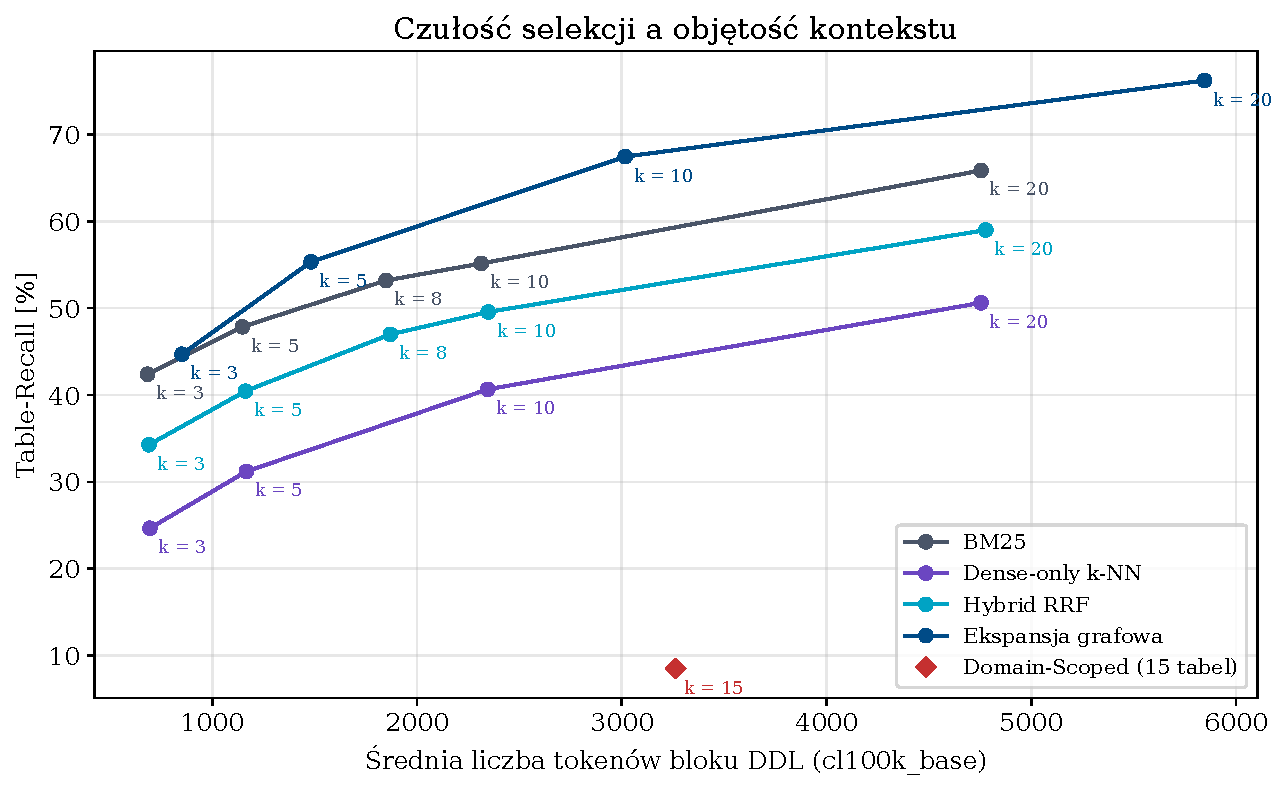
\includegraphics[width=0.85\linewidth]{rysunki/fig_pareto_recall_tokens.pdf}
\caption[Table-Recall a liczba tokenów DDL]{Table-Recall wobec średniej liczby tokenów bloku DDL dla badanych strategii i~wartości $k$ ($N = \wynNQueries$; analiza wtórna pliku \texttt{schema\_retrieval.parquet})}
\label{fig:pareto_recall_tokens}
\end{figure}

\begin{figure}[htbp]
\centering
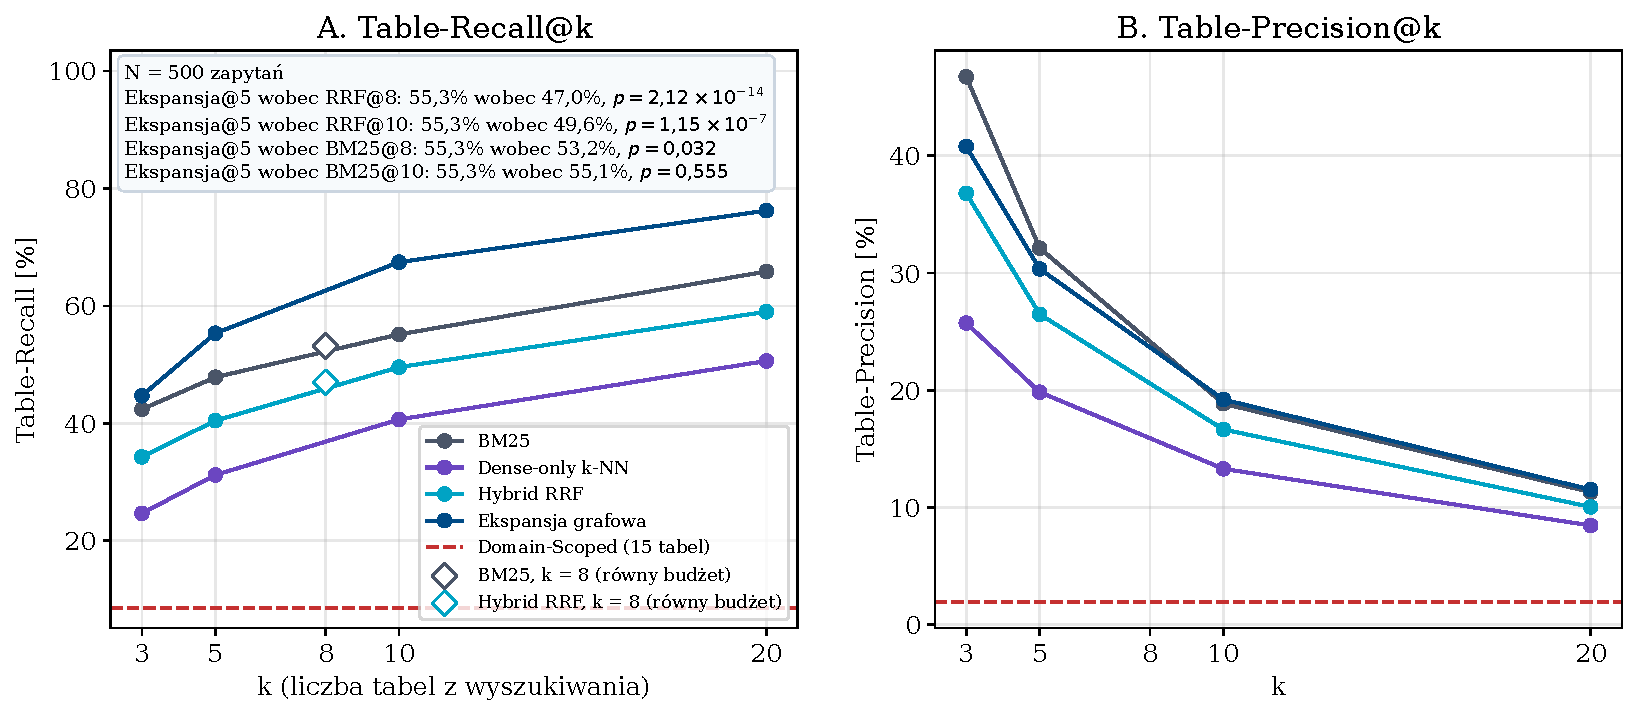
\includegraphics[width=0.88\linewidth]{rysunki/fig_schema_recall_precision.pdf}
\caption[Table-Recall@k oraz Table-Precision@k ($N = 500$)]{Table-Recall@$k$ oraz Table-Precision@$k$ w~funkcji parametru $k \in \{3, 5, 10, 20\}$ dla badanych strategii ($N = \wynNQueries$); wariant autorski zwraca przy danym $k$ więcej tabel niż warianty bazowe}
\label{fig:schema_recall_precision}
\end{figure}

Rysunek~\ref{fig:schema_recall_precision} przedstawia czułość i~precyzję w~funkcji $k$. Wariant autorski ma najwyższą czułość przy każdym $k$ (od \wynRecallGraphThree\% przy $k = 3$ do \wynRecallGraphTwenty\% przy $k = 20$), lecz przy danym $k$ zwraca więcej tabel niż warianty bazowe, więc porównanie przy tym samym $k$ nie jest porównaniem przy równym budżecie. Przy $k = 10$ wariant BM25 osiąga \wynRecallBmTen\%, a~RRF \wynRecallRrfTen\%.

\subsection{Dokładność generacji Text-to-SQL}

Generację SQL wykonano dla $k = 5$ oraz dla wariantów równego budżetu ($k = 8$) na obu profilach modeli, łącznie \wynGenRecords{} wywołań modelu. Tabela~\ref{tab:text2sql_results} i~rysunek~\ref{fig:text2sql_accuracy} przedstawiają odsetki Valid SQL oraz EX z~przedziałami ufności 95\%.

\begin{table}[htbp]
\centering
\small
\caption[Valid SQL oraz EX dla profili 3B i 7B ($N = 500$)]{Odsetek Valid SQL oraz EX [\%] z~95\% przedziałem ufności Cloppera--Pearsona dla profili 3B i~7B ($N = \wynNQueries$ na strategię)}
\label{tab:text2sql_results}
\resizebox{\linewidth}{!}{%
\begin{tabular}{lcccc}
\toprule
\textbf{Strategia} & \multicolumn{2}{c}{\textbf{Profil 3B}} & \multicolumn{2}{c}{\textbf{Profil 7B}} \\
\cmidrule(lr){2-3} \cmidrule(lr){4-5}
 & Valid SQL & EX [95\% CI] & Valid SQL & EX [95\% CI] \\
\midrule
\tabelawynikow{tab_text2sql}
\bottomrule
\end{tabular}%
}
\end{table}

\begin{figure}[htbp]
\centering
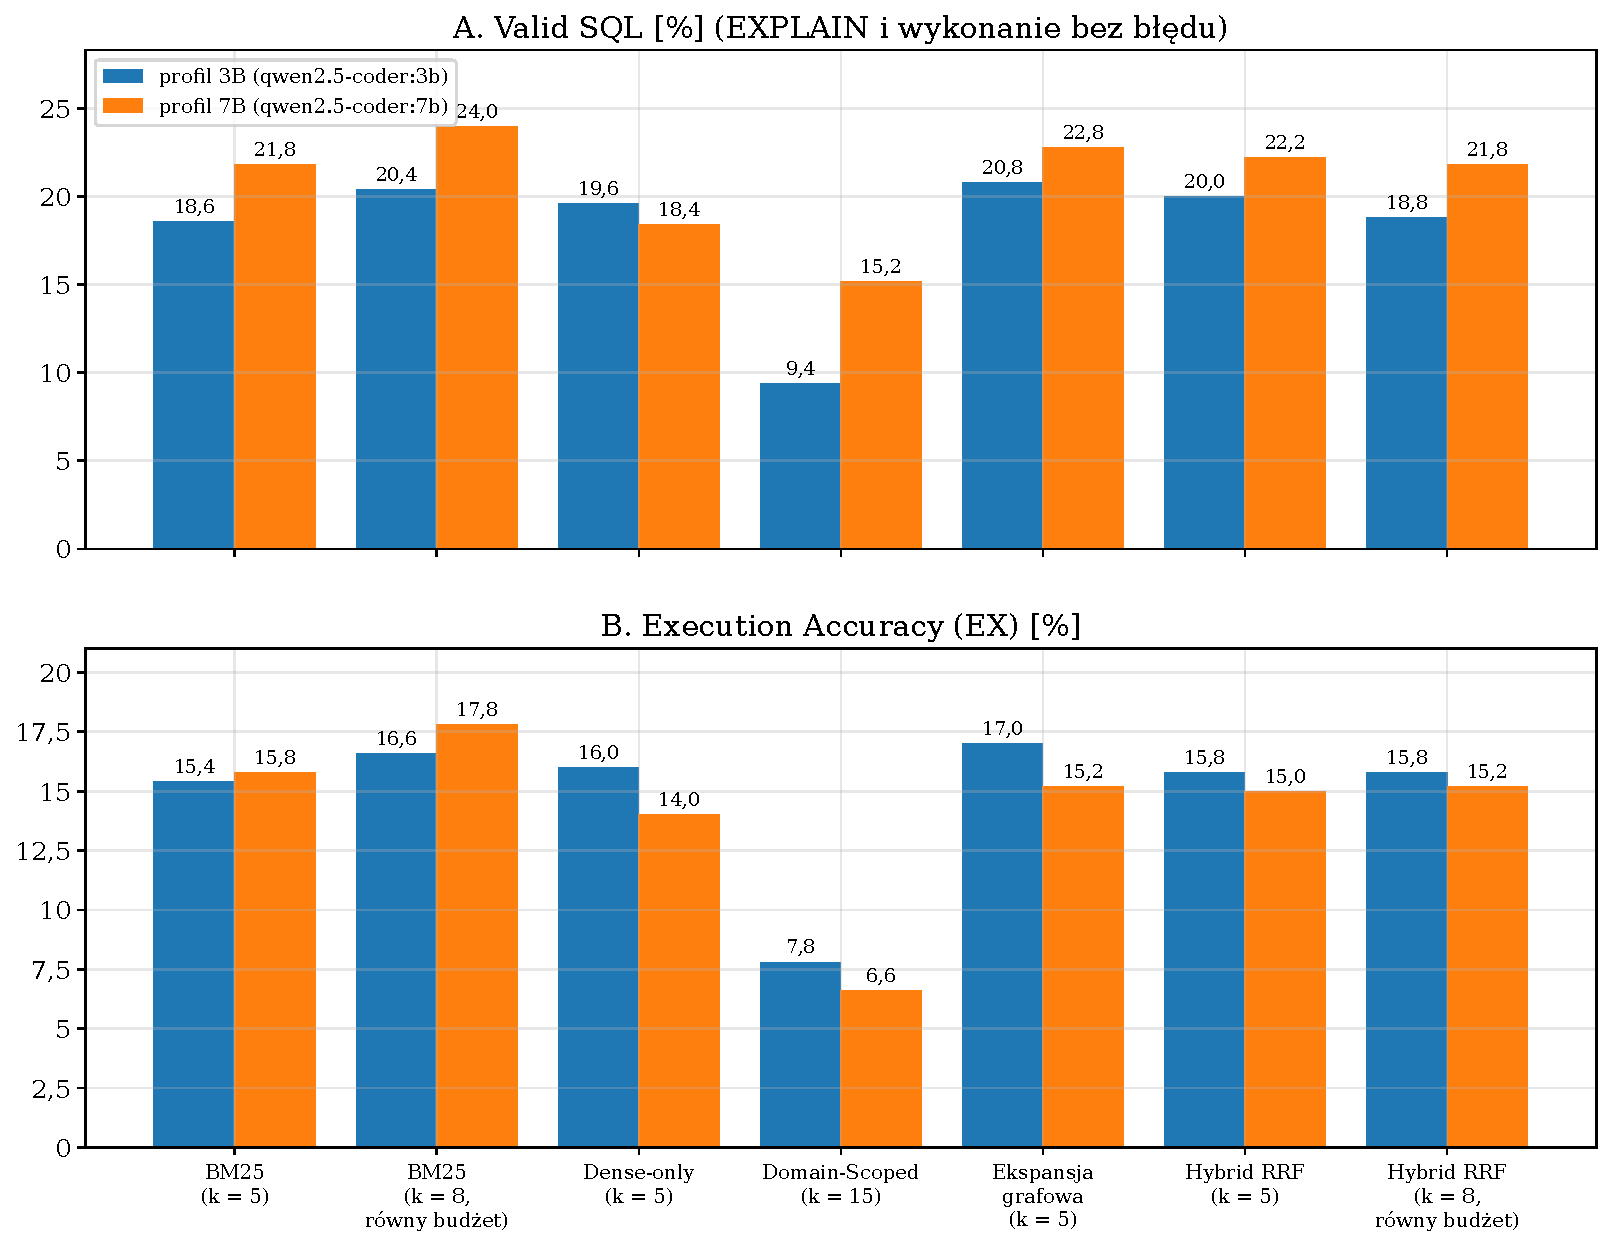
\includegraphics[width=0.88\linewidth]{rysunki/fig_text2sql_accuracy.pdf}
\caption[Valid SQL oraz Execution Accuracy dla profili 3B i 7B]{Valid SQL oraz Execution Accuracy [\%] dla profili 3B (\texttt{qwen2.5-coder:3b}) i~7B (\texttt{qwen2.5-coder:7b}), $N = \wynNQueries$ zapytań na strategię}
\label{fig:text2sql_accuracy}
\end{figure}

Odsetki EX wszystkich strategii selekcyjnych mieszczą się w~wąskim zakresie: na profilu 3B od \wynExSmallBmFive\% (BM25@5) do \wynExSmallGraphFive\% (ekspansja grafowa), a~na profilu 7B od \wynExLargeDenseFive\% (Dense-only) do \wynExLargeBmEight\% (BM25@8); wariant autorski osiąga na profilu 7B \wynExLargeGraphFive\%. Przedziały ufności wszystkich strategii selekcyjnych nakładają się. Wyraźnie niższy wynik daje tylko Domain-Scoped (\wynExSmallDomain\% i~\wynExLargeDomain\%). Profil 7B nie dał systematycznej poprawy EX względem profilu 3B: dla części strategii EX wzrósł, a~dla części spadł.

Tabela~\ref{tab:mcnemar_ex} zestawia dokładne testy McNemara dla EX wariantu autorskiego względem każdej strategii bazowej. Bez korekty na wielokrotne porównania jedyną istotną różnicą między strategiami selekcyjnymi jest przewaga BM25@8 nad wariantem autorskim na profilu 7B (\wynMcLargeBmEightA{} wobec \wynMcLargeBmEightB{} par niezgodnych, $p = \wynMcLargeBmEightP$). Po korekcie Holma w~rodzinie sześciu porównań profilu (analiza wtórna, skrypt \texttt{o2\_holm\_mcnemar.py}) różnica ta przestaje być istotna ($p_{\text{Holm}} = \wynOtwoHolmBmEightLarge$), podobnie jak wszystkie pozostałe różnice między strategiami selekcyjnymi na obu profilach; istotna pozostaje jedynie przewaga nad Domain-Scoped. Dane nie pozwalają więc wskazać strategii selekcyjnej o~wyższej EX w~żadnym kierunku.

\paragraph{Czułość pełna a~EX (analiza wtórna).} Średnia czułość słabo opisuje to, co jest istotne dla generacji: zapytanie może się udać tylko wtedy, gdy wycinek zawiera wszystkie potrzebne tabele. Wariant autorski dostarcza pełny zbiór tabel wzorcowych (Table-Recall = 1) w~\wynOoneFullGraph\% zapytań, wobec \wynOoneFullBmEight\% dla BM25@8 i~\wynOoneFullRrfEight\% dla RRF@8 (skrypt \texttt{o1\_czulosc\_a\_ex.py}). Przy pełnej czułości EX wariantu autorskiego wynosi jednak \wynOoneExFullGraphSmall\% \wynOoneExFullCiGraphSmall{} na profilu 3B i~\wynOoneExFullGraphLarge\% \wynOoneExFullCiGraphLarge{} na profilu 7B, mniej niż dla BM25@8 (\wynOoneExFullBmEightSmall\% i~\wynOoneExFullBmEightLarge\%). Dodatkowe zapytania, dla których ekspansja kompletuje wycinek, to głównie zapytania z~trzema i~więcej tabelami, a~te w~tym zbiorze prawie nigdy nie kończą się poprawnym wynikiem: EX wariantu autorskiego wynosi \wynOoneExGraphLenTwoSmall\% (3B) i~\wynOoneExGraphLenTwoLarge\% (7B) dla ścieżek dwutabelowych, ale tylko \wynOoneExGraphLenThreeSmall\% i~\wynOoneExGraphLenThreeLarge\% dla trzytabelowych i~zero dla dłuższych; podobnie jest dla pozostałych strategii. Wyjaśnia to, dlaczego wyższa czułość nie przekłada się na EX.

\begin{table}[htbp]
\centering
\small
\caption[Testy McNemara dla EX: Graph@5 wobec strategii bazowych]{Dokładny test McNemara dla EX: ekspansja grafowa ($k = 5$) wobec strategii bazowych; $a$ -- liczba zapytań poprawnych tylko dla wariantu autorskiego, $b$ -- tylko dla strategii bazowej ($N = \wynNQueries$); $p_{\text{Holm}}$ -- wartość $p$ po korekcie Holma w~rodzinie sześciu porównań danego profilu (analiza wtórna)}
\label{tab:mcnemar_ex}
\begin{tabular}{llccccc}
\toprule
\textbf{Profil} & \textbf{Strategia bazowa} & \textbf{EX Graph / bazowa [\%]} & $a$ & $b$ & $p$ & $p_{\text{Holm}}$ \\
\midrule
\tabelawynikow{tab_mcnemar}
\bottomrule
\end{tabular}
\end{table}

\subsection{Dekompozycja błędów generacji zapytań}
\label{subsec:wyniki_dekompozycja_ex}

Tabela~\ref{tab:error_taxonomy} i~rysunek~\ref{fig:error_decomposition_tree} przedstawiają rozkład kategorii błędów dla wszystkich strategii i~obu profili.

\paragraph{Wpływ złożoności strukturalnej na Execution Accuracy.} Analiza wtórna rekordów generacji (skrypt \texttt{o9\_klasyfikacja.py}) wykazuje, że zróżnicowanie wskaźnika EX pomiędzy kategoriami zapytań stanowi bezpośrednią konsekwencję ich złożoności strukturalnej. Podczas gdy dla zapytań prostych średnia wartość EX wynosi \wynOnineExSimple\%, w przypadku zapytań średnich (z wielokrotnym złączeniem i agregacją) oraz złożonych (z podzapytaniami CTE, EX równe \wynOnineExComplex\%) wysoki stopień komplikacji relacyjnej i składniowej przekroczył możliwości wnioskowania małych, lokalnych modeli językowych (3B i~7B). Niewielkie modele lokalne mają trudności z poprawną koordynacją wielu predykatów złączeń, klauzul grupowania oraz konstrukcji CTE w rozległym schemacie relacyjnym, co prowadziło do niepoprawności generowanego kodu SQL mimo dostarczenia właściwych struktur tabel w promptcie.

\paragraph{Kategoria \texttt{TABLE\_MISSING}.} Zgodnie z~kolejnością reguł taksonomii rekord trafia do tej kategorii, gdy zapytanie odwołuje się do tabeli spoza wycinka, niezależnie od zgłoszonego błędu. Ponieważ pytania wymieniają nazwy wszystkich tabel, model używa ich także bez otrzymania ich definicji, a~zapytanie kończy się błędem nieistniejącej kolumny (w~\wynOnineTableMissingColumn\% rekordów tej kategorii PostgreSQL zgłosił nieistniejącą kolumnę): model zgaduje nazwę kolumny klucza obcego i~kierunek złączenia. Ręczny przegląd losowej próby 40 rekordów wariantu autorskiego z~EX = fałsz (po 20 na profil, ziarno 2026; plik \texttt{derived/o9\_klasyfikacja\_reczna.csv}) potwierdził ten mechanizm: w~\wynOnineSampleB{} rekordach model użył tabel z~pytania nieobecnych w~wycinku i~błędnie odgadł kolumnę złączenia, w~\wynOnineSampleC{} błędnie odgadł kolumnę lub kierunek złączenia mimo obecności wszystkich tabel, w~\wynOnineSampleD{} błędnie zinterpretował alias z~treści pytania złożonego, a~w~\wynOnineSampleE{} zapytanie było poprawne składniowo, lecz zwracało odmienny zbiór wynikowy. Nie stwierdzono błędów ekstrakcji SQL z~odpowiedzi (wszystkie odpowiedzi zawierały blok kodu, żadna nie została ucięta), więc różnice między profilami nie wynikają z~formatu odpowiedzi.

\begin{table}[htbp]
\centering
\small
\caption[Taksonomia błędów Text-to-SQL]{Liczba rekordów z~EX = fałsz w~kategoriach taksonomii błędów ($N = \wynNQueries$ na strategię i~profil)}
\label{tab:error_taxonomy}
\resizebox{\linewidth}{!}{%
\begin{tabular}{llccccccc}
\toprule
\textbf{Profil} & \textbf{Strategia} & \textbf{EX = fałsz} & \texttt{TABLE\_} & \texttt{COLUMN\_} & \texttt{SEMANTIC\_} & \texttt{JOIN\_} & \texttt{SYNTAX\_} & \texttt{TRUNC.} \\
 & & & \texttt{MISSING} & \texttt{HALLUC.} & \texttt{MISMATCH} & \texttt{COND.} & \texttt{ERROR} & \\
\midrule
\tabelawynikow{tab_taksonomia}
\bottomrule
\end{tabular}%
}
\end{table}

\begin{figure}[htbp]
\centering
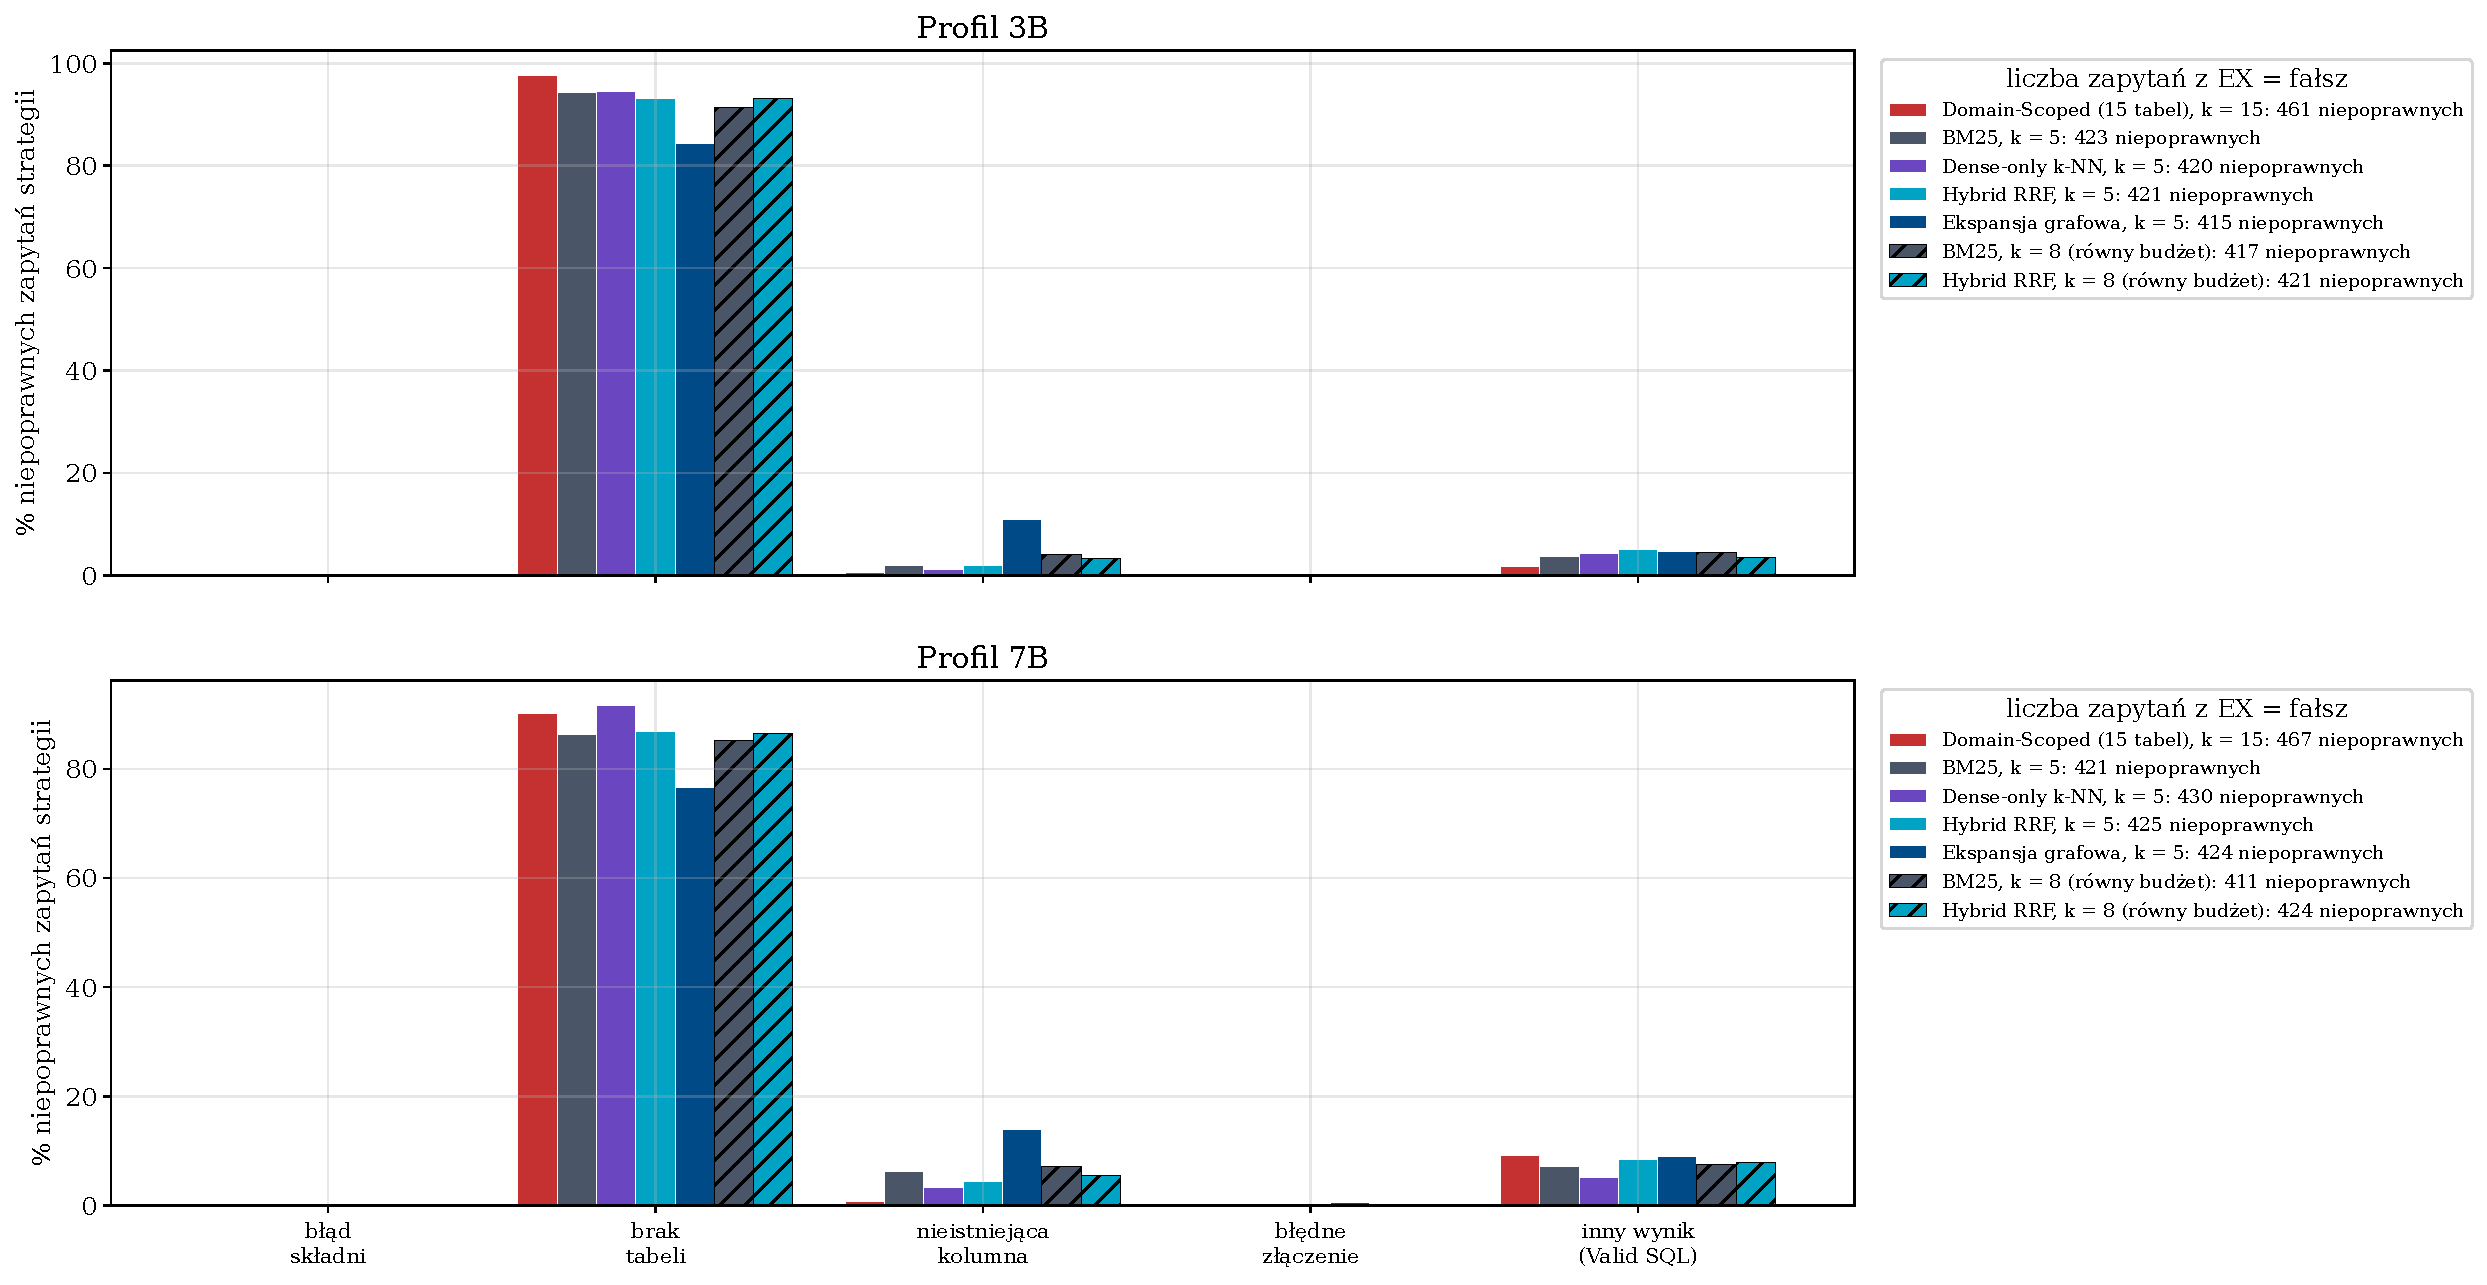
\includegraphics[width=0.88\linewidth]{rysunki/fig_error_decomposition_tree.pdf}
\caption[Dekompozycja przyczyn niepowodzenia zapytań SQL]{Rozkład kategorii błędów (odsetek zapytań z~EX = fałsz danej strategii) dla profili 3B i~7B, łącznie z~wariantami równego budżetu ($k = 8$, kreskowanie); w~legendzie liczba zapytań z~EX = fałsz. Kategoria \texttt{TRUNCATION} nie wystąpiła; kategoria pustego wyniku wzorca (\texttt{GT\_EMPTY}) dotyczy nieważnych próbek i~również nie wystąpiła}
\label{fig:error_decomposition_tree}
\end{figure}

Formalnie dominującą kategorią jest \texttt{TABLE\_MISSING}: dla wariantu autorskiego obejmuje \wynErrTableMissingSmall{} z~\wynErrFalseSmall{} błędnych rekordów na profilu 3B (\wynErrTableMissingPctSmall\%) oraz \wynErrTableMissingLarge{} z~\wynErrFalseLarge{} na profilu 7B (\wynErrTableMissingPctLarge\%). Model odwołuje się więc najczęściej do tabeli spoza dostarczonego wycinka, co jest zgodne z~konstrukcją pytań wymieniających wprost nazwy wszystkich tabel ścieżki: brak dowolnej z~nich w~wycinku kończy się błędem. Na profilu 7B wariant autorski ma \wynErrColumnLarge{} halucynacji kolumn i~\wynErrSemanticLarge{} niezgodności semantycznych, a~błędy predykatu złączenia występują sporadycznie (\wynErrJoinLarge). Kategoria \texttt{TRUNCATION} nie wystąpiła w~żadnej strategii, co jest zgodne z~brakiem rekordów z~podejrzeniem obcięcia kontekstu.

\subsection{Badanie ablacyjne parametru ekspansji grafowej \texorpdfstring{$M_{\text{exp}}$}{Mexp}}
\label{subsec:wyniki_ablation_mexp}

Wpływ maksymalnej liczby tabel mostkujących zbadano dla $M_{\text{exp}} \in \{0, 1, 2, 3, 5\}$ na zbiorze $N = \wynNQueries$ zapytań przy $k = 5$ (rysunek~\ref{fig:ablation_mexp}).

\begin{figure}[htbp]
\centering
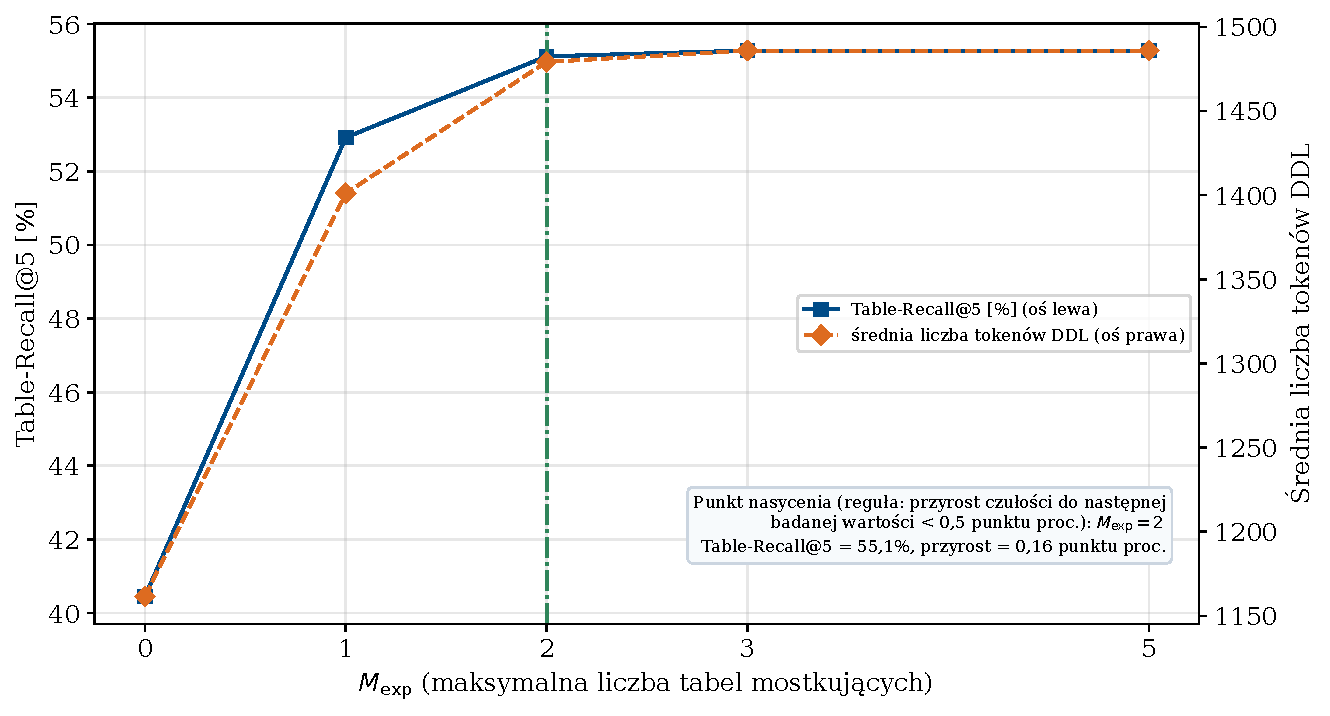
\includegraphics[width=0.88\linewidth]{rysunki/fig_ablation_mexp.pdf}
\caption[Badanie ablacyjne parametru $M_{\text{exp}}$]{Badanie ablacyjne parametru $M_{\text{exp}} \in \{0, 1, 2, 3, 5\}$: Table-Recall@5 oraz średnia liczba tokenów bloku DDL ($N = \wynNQueries$); linia przerywana pionowa wskazuje punkt nasycenia według reguły z~konfiguracji rundy}
\label{fig:ablation_mexp}
\end{figure}

Bez ekspansji ($M_{\text{exp}} = 0$, wynik równy RRF@5) Table-Recall@5 wynosi \wynAbRecallZero\% przy \wynAbDdlZero{} tokenach DDL. Jedna tabela mostkująca podnosi czułość do \wynAbRecallOne\% (\wynAbDdlOne{} tokenów), dwie -- do \wynAbRecallTwo\% (\wynAbDdlTwo{} tokenów), a~$M_{\text{exp}} = 3$ i~$M_{\text{exp}} = 5$ dają identyczne \wynAbRecallThree\% (\wynAbDdlThree{} tokenów). Reguła punktu nasycenia zapisana w~konfiguracji przed pomiarem (najmniejsze $M_{\text{exp}}$, dla którego przyrost względem następnej badanej wartości jest mniejszy niż 0,5 punktu procentowego) wskazuje $M_{\text{exp}} = \wynAbSweet$ (przyrost \wynAbSweetGain~pp). Kod bramy i~pozostałe eksperymenty używają $M_{\text{exp}} = 3$; różnica czułości między wartościami 2 i~3 jest pomijalna, podobnie jak różnica objętości DDL.

Czas pojedynczego wywołania selekcji przy $M_{\text{exp}} = 3$ (mediana i~$p_{95}$ z~$N = \wynNQueries$ wywołań) wyniósł \wynTTotalMed~ms ($p_{95}$ \wynTTotalPnn~ms). Dominuje fuzja RRF z~wyszukiwaniem wektorowym (\wynTRrfMed~ms); załadowanie grafu z~pamięci podręcznej zajęło \wynTGraphMed~ms, wyszukiwanie mostków \wynTBridgeMed~ms ($p_{95}$ \wynTBridgePnn~ms), a~synteza DDL \wynTDdlMed~ms.

\subsection{Czas do pierwszego tokenu w funkcji rozmiaru promptu}
\label{subsec:wyniki_ttft}

W~osobnym eksperymencie zmierzono $TTFT$ dla promptów zawierających bloki DDL o~docelowej objętości od 1000 do 28\,000 tokenów, po \wynTtftReps{} powtórzeń na punkt dla każdego profilu. Okno \texttt{num\_ctx} dobierano do rozmiaru promptu z~zapasem 2048 tokenów, a~do każdego promptu dodawano unikalny identyfikator, aby wyeliminować ponowne użycie pamięci podręcznej prefiksu w~serwerze Ollama. Liczbę tokenów promptu odczytano z~licznika \texttt{prompt\_eval\_count} serwera; w~żadnym pomiarze nie wykryto obcięcia kontekstu. Wyniki przedstawia tabela~\ref{tab:ttft_scaling} i~rysunek~\ref{fig:ttft_scaling}.

\begin{table}[htbp]
\centering
\small
\caption[TTFT w funkcji liczby tokenów promptu]{Mediana $TTFT$ [ms] z~95\% przedziałem ufności (bootstrap), $p_{95}$ $TTFT$ oraz mediana całkowitego czasu żądania $L_{\text{E2E}}$ [ms] w~funkcji liczby tokenów promptu (\wynTtftReps{} powtórzeń na punkt; generacja ograniczona do 64 tokenów)}
\label{tab:ttft_scaling}
\resizebox{\linewidth}{!}{%
\begin{tabular}{rrcccccc}
\toprule
\textbf{Tokeny} & \texttt{num\_ctx} & \multicolumn{3}{c}{\textbf{Profil 3B}} & \multicolumn{3}{c}{\textbf{Profil 7B}} \\
\cmidrule(lr){3-5} \cmidrule(lr){6-8}
\textbf{promptu} & & $TTFT$ [95\% CI] & $p_{95}$ & $L_{\text{E2E}}$ & $TTFT$ [95\% CI] & $p_{95}$ & $L_{\text{E2E}}$ \\
\midrule
\tabelawynikow{tab_ttft}
\bottomrule
\end{tabular}%
}
\end{table}

\begin{figure}[htbp]
\centering
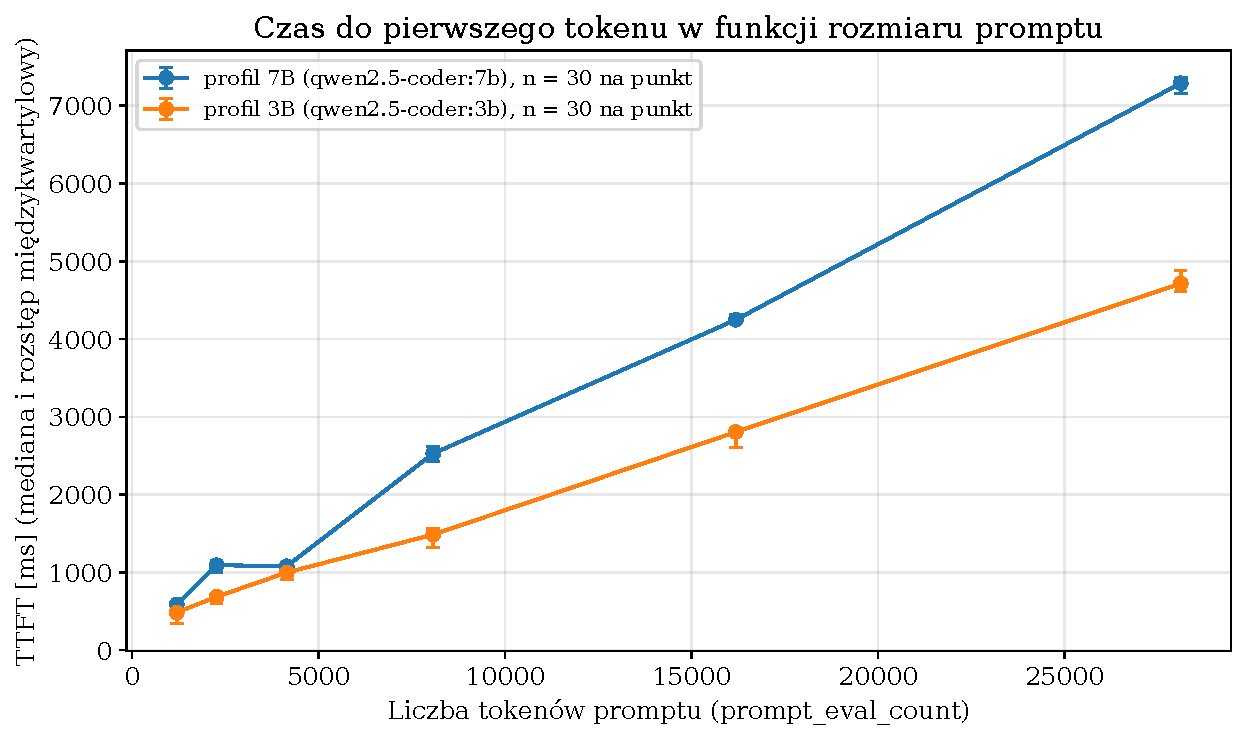
\includegraphics[width=0.88\linewidth]{rysunki/fig_ttft_scaling.pdf}
\caption[TTFT w funkcji liczby tokenów promptu]{Mediana $TTFT$ w~funkcji liczby tokenów promptu (\texttt{prompt\_eval\_count}) dla profili 3B i~7B (\wynTtftReps{} powtórzeń na punkt)}
\label{fig:ttft_scaling}
\end{figure}

$TTFT$ rośnie w~przybliżeniu liniowo z~rozmiarem promptu: nachylenie prostej regresji wynosi \wynTtftSlopeSmall~ms na 1000 tokenów dla profilu 3B (95\% CI \wynTtftSlopeCiSmall) oraz \wynTtftSlopeLarge~ms na 1000 tokenów dla profilu 7B (95\% CI \wynTtftSlopeCiLarge). Dla promptu około \wynTtftPromptLargeOne{} tokenów mediana $TTFT$ wynosi \wynTtftSmallOne~ms (3B) i~\wynTtftLargeOne~ms (7B), a~dla około \wynTtftPromptLargeMax{} tokenów -- \wynTtftSmallMax~ms i~\wynTtftLargeMax~ms. Dla profilu 7B zależność nie jest ściśle monotoniczna między punktami około 2000 i~4000 tokenów (tabela~\ref{tab:ttft_scaling}). Prompty Scenariusza~A (do \wynMaxPromptEval{} tokenów) mieszczą się w~dolnej części badanego zakresu. Pełnego zrzutu DDL (\wynFullDumpTokens{} tokenów) nie da się umieścić w~oknie kontekstu badanych modeli.


%%%%%%%%%%%%%%%%%%%%%%%%%%%%%%%%%%%%%%%%%%%%%%%%%%%%%%%%%%%%%%%%%%%%%%%%%%%%%%%
\section{Analiza progu opłacalności transferu binarnego Out-of-Band (Scenariusz B1)}
\label{sec:wyniki_scenariusz_b1}

\subsection{Warunki pomiaru}

W~Scenariuszu B1 zmierzono czas przekazania ładunku binarnego $S \in [512\ \text{B}; 50\ \text{MiB}]$ (9 rozmiarów, \wynOobReps{} powtórzeń na punkt po 5 przebiegach rozgrzewkowych) w~trzech trybach: In-Band (ładunek zakodowany w~Base64 w~ramce JSON-RPC), OOB przez pamięć współdzieloną POSIX SHM oraz OOB przez obiekt zapisany w~lokalnym magazynie z~deskryptorem zawierającym podpisany URI. Wszystkie operacje nadawcy i~odbiorcy wykonywano w~jednym procesie: ramka JSON-RPC była serializowana i~parsowana w~pamięci, bez przesyłania przez potok \texttt{stdio} ani gniazdo sieciowe, a~obiekt trybu OOB z~URI odbiorca odczytywał bezpośrednio z~pliku. Mierzony czas obejmuje więc koszty obliczeniowe przekazania (kodowanie i~dekodowanie Base64, sumy kontrolne SHA-256 -- w~trybie In-Band dwukrotnie, w~trybie SHM jednokrotnie, bez weryfikacji przy odczycie -- serializację ramki, kopiowanie do segmentu i~z~segmentu, zapis i~odczyt pliku), a~nie transmisję przez kanał MCP. Korzyść z~transferu OOB dotyczy czasu i~zasobów hosta; dane przekazane poza pasmem nie trafiają do okna kontekstu modelu w~żadnym z~trybów, więc pomiar nie dotyczy kosztu tokenowego.

Profil \emph{loopback} zmierzono bezpośrednio na jednym węźle i~wykorzystano jako kalibrację kosztów obliczeniowych. Profile LAN i~WAN stanowią analityczną projekcję parametryczną: do empirycznie zmierzonego czasu kodowania, kopiowania, sum kontrolnych i~serializacji dodano składniki sieciowe wynikające z~RTT, przepustowości i~rozmiaru ramki. Dla In-Band uwzględniono jeden czas RTT oraz czas przesłania ramki ($8 \cdot |\text{ramka}| / B$), a~dla OOB z~URI dwa czasy RTT oraz czasy przesłania deskryptora i~ładunku. Przyjęte parametry to RTT = 1~ms, przepustowość $B$ = 1000~Mb/s i~brak fluktuacji dla LAN oraz RTT = 30~ms, $B$ = 250~Mb/s i~fluktuacja $\pm 2$~ms dla WAN. Progi LAN i~WAN opisują zatem zachowanie modelu skalibrowanego na pojedynczym węźle; bootstrapowy przedział ufności odnosiłby się wyłącznie do zmienności obliczeń lokalnych. Mediany czasów transferu dla wszystkich profili przedstawia rysunek~\ref{fig:oob_crossover_rtt}.

\begin{figure}[htbp]
\centering
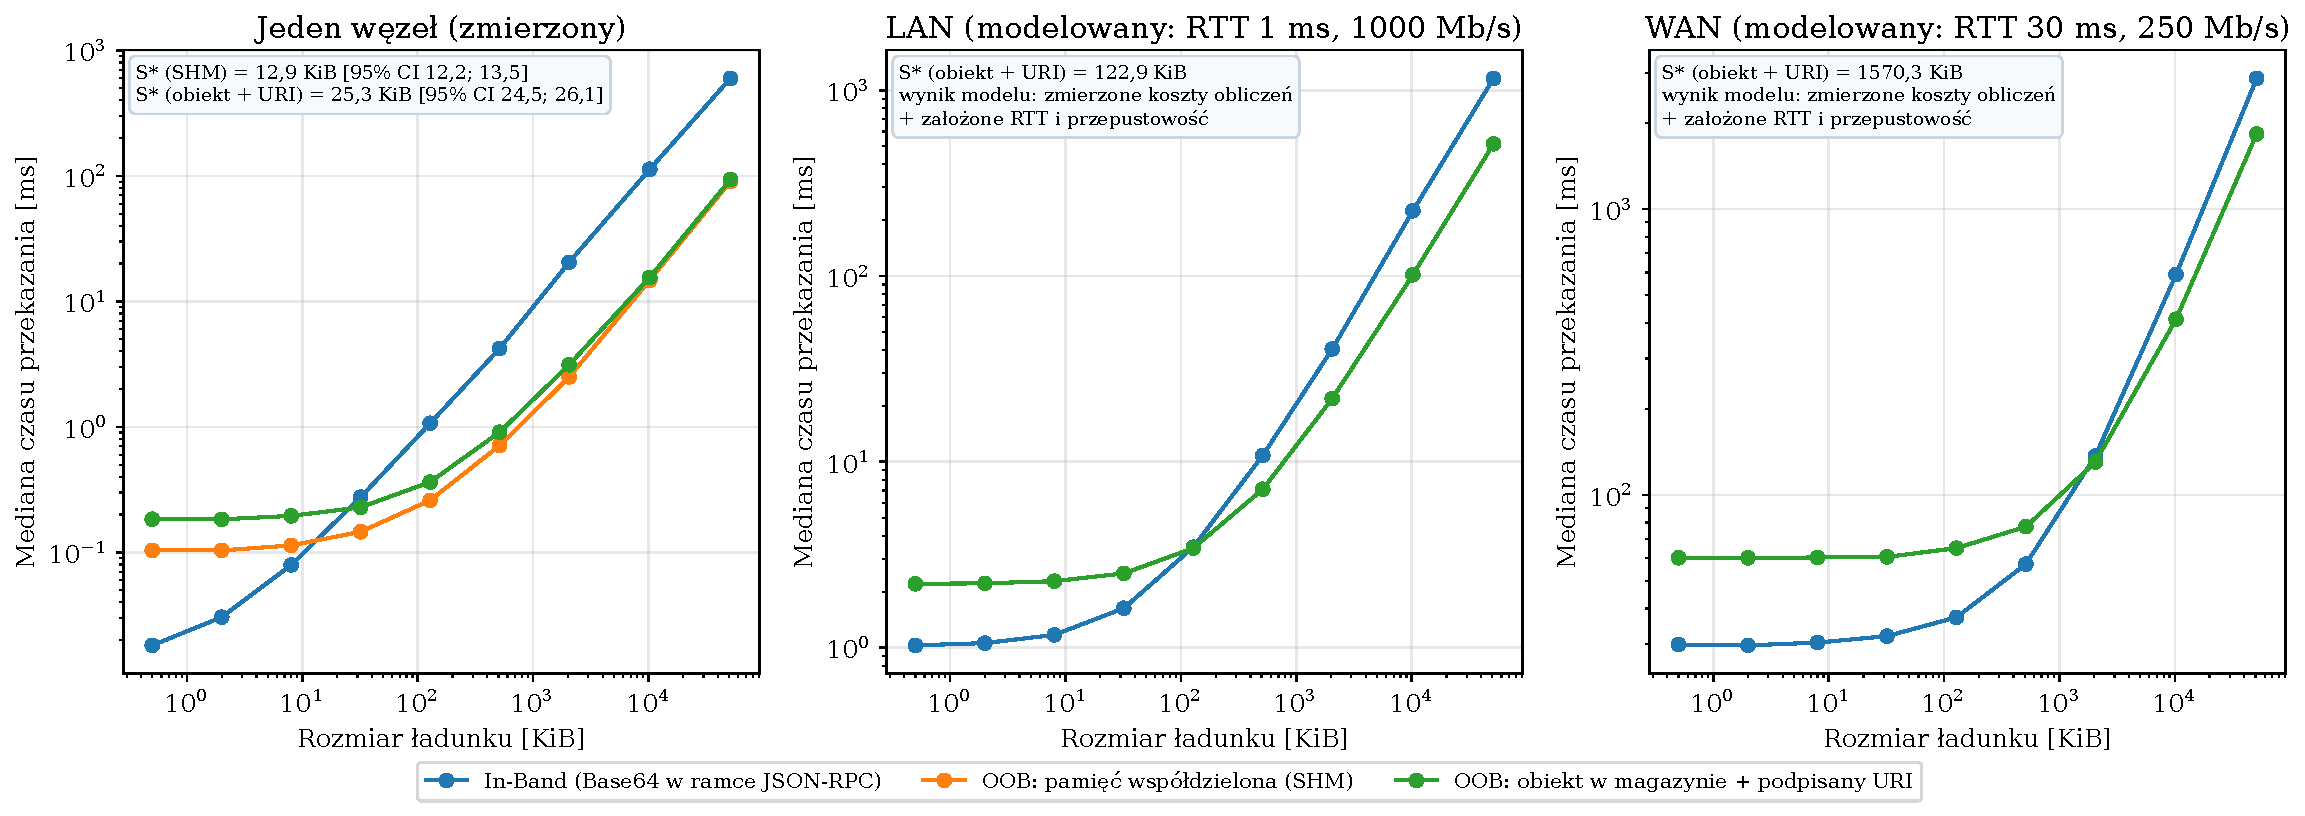
\includegraphics[width=0.88\linewidth]{rysunki/fig_oob_crossover_rtt.pdf}
\caption[Progi opłacalności transferu Out-of-Band]{Mediana czasu przekazania ładunku w~funkcji jego rozmiaru dla trybu In-Band (Base64) i~trybów Out-of-Band (pamięć współdzielona; obiekt w~magazynie z~podpisanym URI). Profil jednego węzła zmierzono; profile LAN (RTT 1~ms, 1000~Mb/s) i~WAN (RTT 30~ms, 250~Mb/s) są wynikiem modelu (zmierzone koszty obliczeń z~dodanym obliczonym czasem sieci), dlatego nie podano dla nich przedziałów ufności}
\label{fig:oob_crossover_rtt}
\end{figure}

\subsection{Punkty przecięcia}

Punkt przecięcia $S^*$ wyznaczono jako przecięcie prostych dopasowanych do median czasów dwóch trybów w~otoczeniu zmiany znaku różnicy (po dwa sąsiednie rozmiary), a~przedział ufności -- bootstrapem powtórzeń (tylko dla profilu zmierzonego). Wyniki zestawia tabela~\ref{tab:oob_sstar}.

\begin{table}[htbp]
\centering
\small
\caption[Punkty przecięcia $S^*$ transferu OOB i In-Band]{Rozmiar ładunku $S^*$ [KiB], powyżej którego tryb OOB jest szybszy od In-Band Base64 (95\% CI bootstrap)}
\label{tab:oob_sstar}
\begin{tabular}{llllcc}
\toprule
\textbf{Profil} & \textbf{Tryb OOB} & \textbf{Tryb pomiaru} & \textbf{Parametry sieci} & $S^*$ [KiB] & \textbf{95\% CI} \\
\midrule
\tabelawynikow{tab_sstar}
\bottomrule
\end{tabular}
\end{table}

\begin{equation}
S^*_{\text{loopback, SHM}} = \wynSstarLoopShm\ \text{KiB}
\label{eq:empiryczny_crossover}
\end{equation}

Na jednym węźle pamięć współdzielona jest szybsza od In-Band od ok. \wynSstarLoopShm~KiB, a~OOB z~obiektem w~magazynie -- od ok. \wynSstarLoopHttp~KiB. Dla ładunku 50~MiB mediana czasu wynosi \wynFiftyShm~ms dla SHM wobec \wynFiftyInband~ms dla In-Band, czyli \wynSpeedupFifty-krotną różnicę. W~trybie In-Band przy 50~MiB samo kodowanie Base64 zajmuje \wynFiftyEnc~ms, dekodowanie \wynFiftyDec~ms, a~każde obliczenie SHA-256 \wynFiftySha~ms; kopiowanie do segmentu SHM zajmuje \wynFiftyShmCopy~ms. Narzut ramki In-Band względem ładunku dąży do \wynFrameOverheadTen\% (przy 10~MiB), co odpowiada teoretycznemu narzutowi Base64 (4/3), a~dla ładunków 512~B wynosi \wynFrameOverheadSmall\% z~powodu stałej części ramki JSON-RPC. W~modelu LAN próg rośnie do \wynSstarLan~KiB, a~w~modelu WAN do \wynSstarWan~KiB, ponieważ dodatkowa runda sieciowa trybu OOB z~URI jest amortyzowana dopiero przy dużych ładunkach.

\paragraph{Walidacja modelu progu (analiza wtórna).} Wzór~\eqref{eq:crossover_shm_formula} zweryfikowano składowymi czasów zarejestrowanymi w~rundzie (skrypt \texttt{o7\_model\_sstar.py}). Z~median składowych dla rozmiarów od 512~B do 128~KiB wyznaczono metodą najmniejszych kwadratów przepustowości operacji oraz stałe narzuty (tabela~\ref{tab:oob_model}). Podstawienie do wzoru daje $S^*_{\text{SHM}} = \wynOsevenModel$~KiB, w~granicach przedziału ufności wartości empirycznej (\wynSstarLoopShm~KiB, 95\% CI \wynSstarCiLoopShm). Zgodność ta potwierdza spójność modelu z~implementacją, lecz nie jest niezależną walidacją, ponieważ parametry pochodzą z~tych samych pomiarów. Składnik resztowy ścieżki In-Band (serializacja i~parsowanie ramki JSON oraz narzut wywołań) odpowiada za \wynOsevenResidShare\% jej kosztu jednostkowego, a~więc za znaczną część przewagi trybu OOB. Gdyby odczyt z~segmentu SHM obejmował weryfikację skrótu (jak w~funkcji \texttt{retrieve}), model daje próg \wynOsevenModelVerify~KiB, poza przedziałem ufności pomiaru; asymetria ścieżek pomiarowych przesuwa więc zmierzony próg w~stronę mniejszych ładunków.

\begin{table}[htbp]
\centering
\small
\caption[Parametry modelu progu $S^*$ wyznaczone ze składowych czasów]{Parametry modelu progu $S^*$ wyznaczone ze składowych czasów rundy (profil jednego węzła, MNK na medianach dla 512~B--128~KiB; analiza wtórna)}
\label{tab:oob_model}
\begin{tabular}{lc}
\toprule
\textbf{Parametr} & \textbf{Wartość} \\
\midrule
$v_{\text{enc}}$ (kodowanie Base64) & \wynOsevenVEnc~MiB/s \\
$v_{\text{dec}}$ (dekodowanie Base64) & \wynOsevenVDec~MiB/s \\
$v_{\text{sha}}$ (SHA-256) & \wynOsevenVSha~MiB/s \\
$v_{\text{json}}$ (składnik resztowy In-Band) & \wynOsevenVJson~MiB/s \\
$v_{\text{copy}}$ / $v_{\text{read}}$ (segment SHM) & \wynOsevenVCopy{} / \wynOsevenVRead~MiB/s \\
$\delta_{\text{IB}}$ / $\delta_{\text{SHM}}$ & \wynOsevenDeltaIb{} / \wynOsevenDeltaShm~$\mu$s \\
$S^*_{\text{SHM}}$: model / pomiar & \wynOsevenModel{} / \wynSstarLoopShm~KiB \\
\bottomrule
\end{tabular}
\end{table}

Hipotezę H2 zweryfikowano na profilu jednego węzła testem Manna--Whitneya dla rozmiaru poniżej i~powyżej progu (tabela~\ref{tab:wilcoxon_hypothesis_tests}). Dla 2~KiB In-Band jest szybszy (mediana \wynHdwaSmallInband~ms wobec \wynHdwaSmallShm~ms dla SHM, $p = \wynHdwaSmallP$), a~dla 10~MiB szybszy jest SHM (\wynHdwaBigShm~ms wobec \wynHdwaBigInband~ms, $p = \wynHdwaBigP$; różnica median 95\% CI \wynHdwaBigCi~ms). W~obu przypadkach rozkłady nie zachodzą na siebie ($|r| = 1$). Wynik ten jest jednak przesądzony konstrukcyjnie: rozmiary odległe o~rzędy wielkości od progu dają rozkłady rozdzielone, więc test potwierdza jedynie istnienie progu w~badanym przedziale. Właściwą miarą jest położenie progu, czyli $S^*$ z~przedziałem ufności oraz jego zgodność z~modelem.

\subsection{Reguła architektoniczna}
\emph{Przy kolokacji agenta i~bazy na jednym węźle transfer przez pamięć współdzieloną jest korzystniejszy dla ładunków większych niż kilkanaście kilobajtów (zmierzony próg \wynSstarLoopShm~KiB). W~środowiskach rozproszonych próg rośnie z~opóźnieniem sieci; według modelu z~przyjętymi parametrami wynosi ok. \wynSstarLan~KiB dla LAN i~ok. \wynSstarWan~KiB dla WAN, przy czym wartości te wymagają potwierdzenia pomiarem w~rzeczywistej sieci.}


%%%%%%%%%%%%%%%%%%%%%%%%%%%%%%%%%%%%%%%%%%%%%%%%%%%%%%%%%%%%%%%%%%%%%%%%%%%%%%%
\section{Paginacja, obciążenie współbieżne i bilans zasobów (Scenariusze B2 \& C1)}
\label{sec:wyniki_scenariusz_b2}

\subsection{Skalowalność paginacji na wolumenie 1 000 000 rekordów}
\label{subsec:wyniki_paginacja_glebokosc}

Opóźnienie pobrania strony 50 rekordów zmierzono na relacji 1~000~000 wierszy (\texttt{public.analytics\_orders}) dla porządku \texttt{created\_at DESC NULLS LAST, amount ASC NULLS LAST, id ASC} wspieranego kompozytowym indeksem B-drzewa, dla dziesięciu offsetów od 0 do 950\,000 wierszy (95\% tabeli), po \wynPagReps{} powtórzeń na punkt i~2 przebiegach rozgrzewkowych. Porównano warianty Indexed Keyset B-Tree, Offset/Limit oraz Unindexed Keyset (z~wyłączonym skanem indeksu, mierzony do offsetu 50\,000, ponieważ każde żądanie wymaga pełnego skanu relacji). Przebieg opóźnień przedstawia rysunek~\ref{fig:pagination_depth_1m}, a~mediany -- tabela~\ref{tab:pagination_depth_summary}.

\begin{figure}[htbp]
\centering
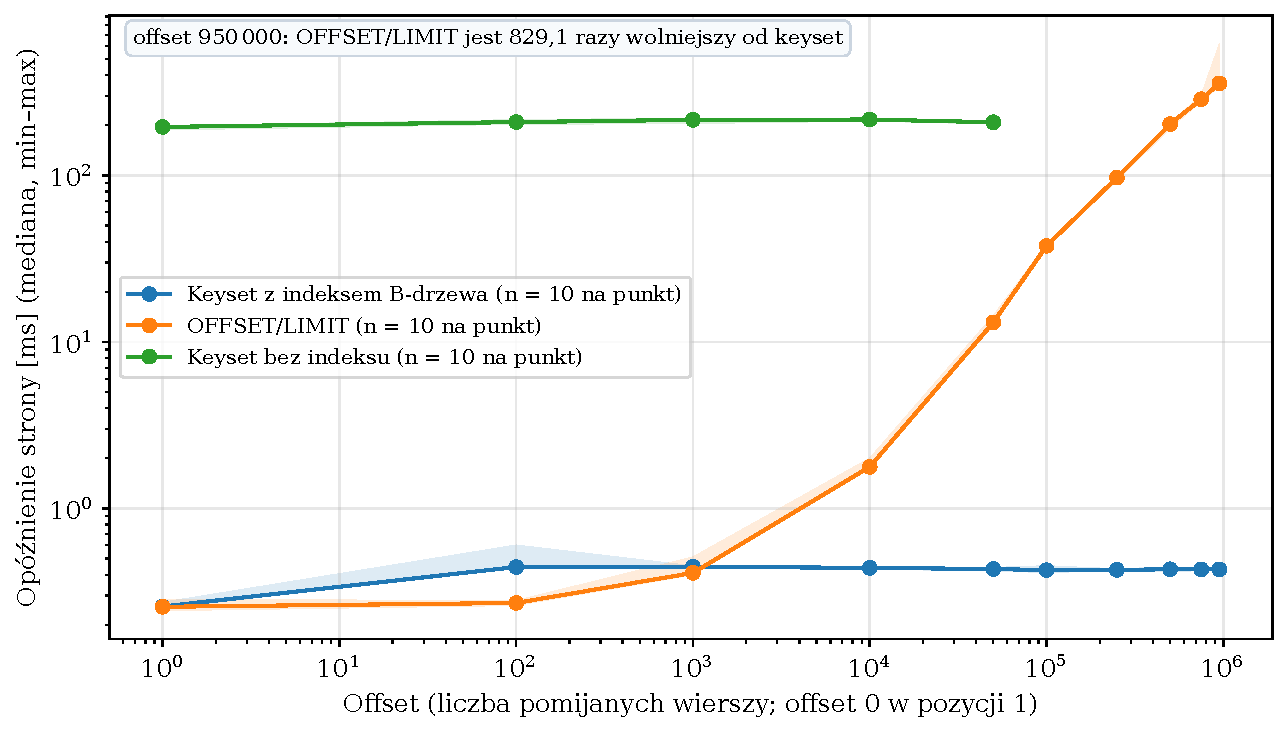
\includegraphics[width=0.92\linewidth]{rysunki/fig_pagination_depth_1m.pdf}
\caption[Opóźnienie paginacji w funkcji offsetu na 1 mln rekordów]{Opóźnienie pobrania strony 50 rekordów w~funkcji offsetu (do 950\,000 wierszy) dla paginacji keyset z~indeksem B-drzewa, OFFSET/LIMIT oraz keyset bez indeksu (skala log-log; mediana i~zakres min--max z~\wynPagReps{} powtórzeń). Offset 0 (pierwsza strona) narysowano w~pozycji 1, ponieważ skala logarytmiczna nie obejmuje zera}
\label{fig:pagination_depth_1m}
\end{figure}

\begin{table}[htbp]
\centering
\small
\caption[Mediany opóźnień paginacji w funkcji offsetu]{Mediany opóźnień pobrania strony 50 rekordów [ms] w~funkcji offsetu $M$ na relacji 1 mln rekordów (\wynPagReps{} powtórzeń na punkt; ,,--'' -- brak pomiaru wariantu nieindeksowanego)}
\label{tab:pagination_depth_summary}
\begin{tabular}{rrcccc}
\toprule
\textbf{Offset $M$} & \textbf{Strona $k$} & \textbf{Indexed Keyset} & \textbf{Offset/Limit} & \textbf{Unindexed Keyset} & \textbf{Offset / Keyset} \\
\midrule
\tabelawynikow{tab_paginacja}
\bottomrule
\end{tabular}
\end{table}

Wyniki z~tabeli~\ref{tab:pagination_depth_summary}:
\begin{itemize}
    \item \textbf{Indexed Keyset B-Tree} zachowuje stałe opóźnienie: przy offsecie 950\,000 mediana wynosi \wynKeysetDeep~ms (\wynKeysetFirst~ms dla pierwszej strony). Nachylenie prostej regresji względem offsetu (\wynKeysetSlope~ms na 100\,tys. wierszy) nie różni się istotnie od zera ($p = \wynKeysetSlopeP$), co jest zgodne z~kosztem $\mathcal{O}(\log N + K)$;
    \item \textbf{Offset/Limit} degraduje się liniowo: nachylenie wynosi \wynOffsetSlope~ms na 100\,tys. pominiętych wierszy ($R^2 = \wynOffsetRsq$), a~przy $M = 950\,000$ mediana sięga \wynOffsetDeep~ms (zakres \wynOffsetDeepMin--\wynOffsetDeepMax~ms), czyli \wynRatioDeep{} razy więcej niż keyset;
    \item dla płytkich offsetów ($M \le 1000$) oba warianty mają porównywalne opóźnienie, a~przewaga keyset rośnie z~głębokością;
    \item \textbf{Unindexed Keyset} ma stałe, wysokie opóźnienie \wynUnidxMin--\wynUnidxMax~ms (mediana \wynUnidxMed~ms) niezależnie od offsetu, ponieważ każde żądanie wymaga skanu sekwencyjnego i~sortowania miliona wierszy. Uzasadnia to moduł \texttt{IndexCatalogGuard}, który wykrywa brak zgodnego indeksu i~ogranicza rozmiar paczki.
\end{itemize}
Bezwzględne czasy zależą od sprzętu, natomiast kształt zależności (stała dla keyset, liniowa dla OFFSET) wynika z~algorytmów.

\subsection{Wpływ postaci predykatu kursorowego na plan wykonania}
\label{subsec:wyniki_predykat}

Porównano dwie postaci predykatu kursorowego dla porządku mieszanego z~\texttt{NULLS LAST}: pojedynczą klauzulę \texttt{WHERE} w~postaci DNF z~operatorami \texttt{OR} (równanie~\eqref{eq:keyset_dnf}) oraz rozłączne gałęzie koniunkcyjne łączone operatorem \texttt{UNION ALL} (podrozdziały~\ref{subsec:projekt_keyset_formalizacja} i~\ref{sec:smart_pagination}). Pomiar wykonano w~tej samej rundzie, na tej samej relacji (\wynPagReps{} powtórzeń na punkt). Tabela~\ref{tab:pagination_predicate_ablation} podaje mediany opóźnień, a~tabela~\ref{tab:pagination_explain} -- parametry planów wykonania (\texttt{EXPLAIN (ANALYZE, BUFFERS)}).

\begin{table}[htbp]
\centering
\small
\caption[Wpływ postaci predykatu kursorowego na opóźnienie keyset]{Mediana opóźnienia paginacji keyset [ms] dla predykatu DNF (\texttt{OR}) oraz rozłącznych gałęzi \texttt{UNION ALL} (\wynPagReps{} powtórzeń na punkt)}
\label{tab:pagination_predicate_ablation}
\begin{tabular}{rccc}
\toprule
\textbf{Offset $M$} & \textbf{Keyset (DNF, \texttt{OR})} & \textbf{Keyset (\texttt{UNION ALL})} & \textbf{DNF / \texttt{UNION ALL}} \\
\midrule
\tabelawynikow{tab_predykat}
\bottomrule
\end{tabular}
\end{table}

\begin{table}[htbp]
\centering
\small
\caption[Plany wykonania predykatów DNF i UNION ALL]{Parametry planów wykonania dla predykatu DNF i~\texttt{UNION ALL}: czas wykonania [ms], liczba wierszy odrzuconych przez filtr, liczba stron bufora (\texttt{shared hit + read}) oraz liczba węzłów z~\texttt{Index Cond}}
\label{tab:pagination_explain}
\begin{tabular}{rcccccc}
\toprule
\textbf{Offset $M$} & \multicolumn{3}{c}{\textbf{DNF (\texttt{OR})}} & \multicolumn{3}{c}{\textbf{\texttt{UNION ALL}}} \\
\cmidrule(lr){2-4} \cmidrule(lr){5-7}
 & Czas & Rows Removed & Strony & Czas & Index Cond & Strony \\
\midrule
\tabelawynikow{tab_explain}
\bottomrule
\end{tabular}
\end{table}

Planer PostgreSQL nie wykorzystuje alternatywy \texttt{OR} jako warunku indeksowego: plan dla DNF zawiera skan indeksu z~filtrem, który przy $M = 950\,000$ odrzuca \wynExplainDnfRemoved{} wierszy i~odczytuje \wynExplainDnfBuf{} stron bufora (\wynExplainDnfMs~ms). W~wariancie \texttt{UNION ALL} każda z~\wynExplainUnionIdx{} gałęzi ma prosty warunek używany jako \texttt{Index Cond}, a~węzeł \texttt{Merge Append} scala posortowane wyniki; plan odczytuje \wynExplainUnionBuf{} stron (\wynExplainUnionMs~ms). Mediana opóźnienia przy $M = 950\,000$ wynosi \wynDnfDeep~ms dla DNF wobec \wynUnionDeep~ms dla \texttt{UNION ALL}. Sama obecność kompozytowego indeksu nie wystarcza więc do uzyskania kosztu $\mathcal{O}(\log N + K)$ -- konieczna jest postać predykatu rozpoznawana przez planer jako warunek indeksowy. Poprawność zapytań wielogałęziowych potwierdzono porównaniem \wynConsSamples{} kolejnych rekordów z~pełnym skanem referencyjnym (pełna zgodność sekwencji, brak duplikatów i~pominięć). Test izolacji migawkowej z~rundy (wstawienie jednego wiersza między pobraniem pierwszej i~drugiej strony z~użyciem migawki) nie wykazał rekordu fantomowego, lecz nie ma mocy rozstrzygającej: wstawiony wiersz miał znacznik \texttt{created\_at = NOW()}, więc przy porządku \texttt{created\_at DESC} trafiłby przed granicę pierwszej strony i~nie pojawiłby się na drugiej stronie także bez migawki. Izolacji migawkowej nie należy zatem uważać za zweryfikowaną pomiarem. Kolumny sortowania relacji \texttt{analytics\_orders} mają ograniczenie \texttt{NOT NULL}, więc test zgodności nie obejmował wartości \texttt{NULL} na granicy strony; wynik zgodności pozostaje ważny dla tych danych, a~poprawność predykatu przy wartościach \texttt{NULL} sprawdzono osobno testem jednostkowym na kodzie w~wersji z~rundy (podrozdział~\ref{subsec:projekt_keyset_formalizacja}), bez pomiaru wydajności.

\subsection{Odporność na obciążenie wieloagentowe i profilowanie zasobów}
\label{sec:wyniki_scenariusz_c1}

W~Scenariuszu C1 obciążenie generowało $M \in \{1, 5, 10, 25, 50, 100, 500\}$ zadań asyncio (klientów) w~jednym procesie, każde wywołujące walidację kolejnego zapytania SQL po zakończeniu poprzedniej (pętla zamknięta; walidator wywoływany bezpośrednio, bez warstwy HTTP; 30~s pomiaru po 5~s rozgrzewki). Porównano trzy warianty wykonania walidacji AST: SYNC (w~wątku pętli zdarzeń), THREAD (pula wątków) oraz POOL (pula procesów \texttt{ProcessPoolExecutor}), domyślnie z~4 pracownikami; przy $M = 100$ zbadano także 2 i~8 pracowników. Pamięć mierzono jako szczytową sumę PSS całego drzewa procesów bramy. Wyniki przedstawia tabela~\ref{tab:concurrency_summary} i~rysunek~\ref{fig:concurrency_rps_lag}.

\begin{table}[htbp]
\centering
\small
\caption[Wpływ obciążenia współbieżnego $M$ na parametry bramy]{Przepustowość (RPS), liczba próbek sondy, mediana, $p_{95}$ i~$p_{99}$ opóźnienia pętli zdarzeń [ms] oraz szczytowa suma PSS drzewa procesów [GiB] w~funkcji liczby klientów $M$ (THREAD i~POOL z~4 pracownikami, o~ile nie podano inaczej)}
\label{tab:concurrency_summary}
\resizebox{\linewidth}{!}{%
\begin{tabular}{lccccccc}
\toprule
\textbf{Wariant} & $M$ & \textbf{RPS} & \textbf{Próbki} & \textbf{Lag $p_{50}$} & \textbf{Lag $p_{95}$} & \textbf{Lag $p_{99}$} & \textbf{PSS [GiB]} \\
\midrule
\tabelawynikow{tab_wspolbieznosc}
\bottomrule
\end{tabular}%
}
\end{table}

\begin{figure}[htbp]
\centering
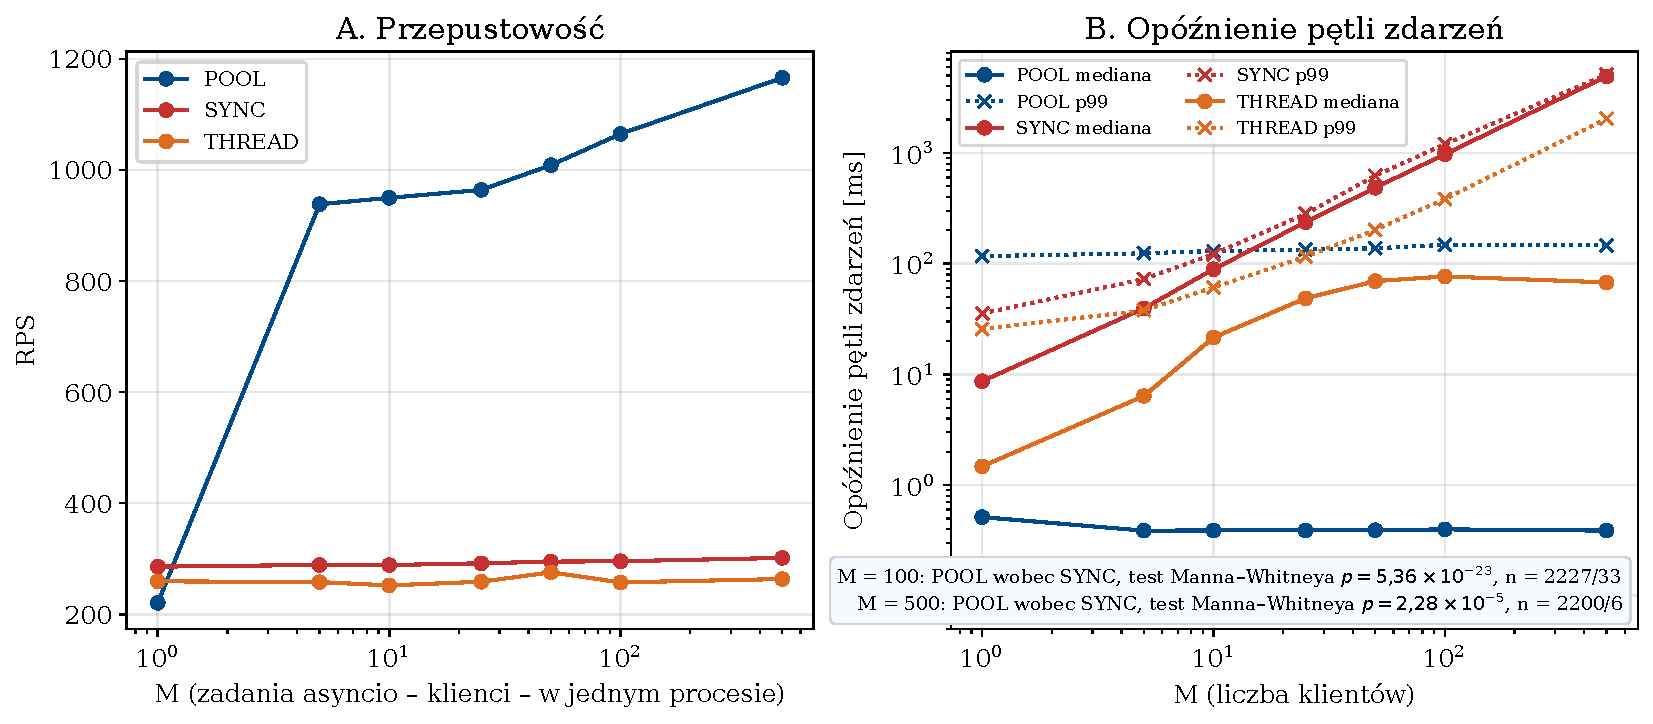
\includegraphics[width=0.88\linewidth]{rysunki/fig_concurrency_rps_lag.pdf}
\caption[Przepustowość oraz opóźnienie pętli zdarzeń pod obciążeniem współbieżnym]{Przepustowość (RPS) oraz mediana i~$p_{99}$ opóźnienia pętli zdarzeń w~funkcji liczby klientów $M$ (zadań asyncio w~jednym procesie) dla wariantów SYNC, THREAD i~POOL (4 pracowników); adnotacja podaje wyniki testu Manna--Whitneya dla H3}
\label{fig:concurrency_rps_lag}
\end{figure}

Wyniki:
\begin{itemize}
    \item \textbf{SYNC:} parsowanie AST w~wątku pętli zdarzeń ogranicza przepustowość do ok. \wynCcSyncHundredRps{} RPS niezależnie od $M$, a~mediana opóźnienia pętli rośnie z~\wynCcSyncOneLagMed~ms przy $M = 1$ do \wynCcSyncHundredLagMed~ms przy $M = 100$ i~\wynCcSyncFivehundredLagMed~ms przy $M = 500$. Przy dużym $M$ sonda zdążyła zarejestrować tylko \wynCcSyncHundredLagN{} i~\wynCcSyncFivehundredLagN{} próbek, ponieważ pętla była zablokowana przez większość czasu pomiaru;
    \item \textbf{THREAD:} przeniesienie parsowania do puli wątków obniża medianę opóźnienia pętli (\wynCcThreadHundredLagMed~ms przy $M = 100$), lecz nie zwiększa przepustowości (\wynCcThreadHundredRps{} RPS), a~zwiększenie liczby wątków do 8 jej nie poprawia (tabela~\ref{tab:concurrency_summary}), co jest zgodne z~serializacją kodu Pythona przez blokadę GIL;
    \item \textbf{POOL:} pula procesów zwiększa przepustowość do \wynCcPoolHundredRps{} RPS przy $M = 100$ i~\wynCcPoolFivehundredRps{} RPS przy $M = 500$, przy medianie opóźnienia pętli \wynCcPoolHundredLagMed~ms i~\wynCcPoolFivehundredLagMed~ms. Zarejestrowany ogon rozkładu jest wyższy: $p_{99}$ wynosi \wynCcPoolHundredLagPnn~ms przy $M = 100$ i~\wynCcPoolFivehundredLagPnn~ms przy $M = 500$; jego przyczynę omówiono niżej. Przy jednym kliencie POOL jest wolniejszy od SYNC (\wynCcPoolOneRps{} wobec \wynCcSyncOneRps{} RPS) z~powodu kosztu komunikacji międzyprocesowej. Przepustowość skaluje się z~liczbą pracowników: \wynCcPoolWTwoRps{} RPS dla 2 i~\wynCcPoolWEightRps{} RPS dla 8 pracowników przy $M = 100$;
    \item \textbf{Bilans pamięci:} szczytowa suma PSS drzewa procesów wynosi ok. \wynCcSyncHundredMem~GiB dla SYNC, \wynCcThreadHundredMem~GiB dla THREAD i~\wynCcPoolHundredMem~GiB dla POOL z~4 pracownikami (\wynCcPoolWEightMem~GiB z~8 pracownikami). Różnica odpowiada ok. \wynCcPoolPerWorker~GiB na proces roboczy. Jako obserwację architektoniczną należy odnotować, że procesy robocze puli dziedziczyły pełen kontekst modułów bramy (\texttt{src.mcp\_server}), w~tym instancję silnika selekcji schematu i~zależności uczenia maszynowego. Wyznacza to prosty i~naturalny kierunek optymalizacji modularnej w~kolejnych wydaniach systemu poprzez odizolowanie lekkiego modułu walidatora AST.
\end{itemize}
\paragraph{Przyczyna ogona $p_{99}$ w~wariancie POOL (analiza wtórna).} Podwyższony ogon $p_{99}$ w~profilowaniu asynchronicznym wariantu POOL ujawnił narzut instrumentacji pomiarowej, zidentyfikowany i~odseparowany w~analizie wtórnej profilu czasowego: próbnik aparatury periodycznie i~synchronicznie odpytywał metryki PSS procesów (wywołanie \texttt{psutil.memory\_full\_info} co 0,5~s w~wątku pętli zdarzeń). W~wariancie POOL przy $M = 100$ wszystkie \wynObSpikesHundred{} próbki sondy z~opóźnieniem powyżej 50~ms pokrywają się z~próbkami pamięci (przy $M = 500$: \wynObSpikesNearFivehundred{} z~\wynObSpikesFivehundred), a~wielkość tych opóźnień rośnie z~liczbą procesów potomnych (próbki $p_{99}$ wynoszą \wynObPnnAllTwoHundred{}, \wynObPnnAllHundred{} i~\wynObPnnAllEightHundred~ms dla \wynObChildrenTwoHundred, \wynObChildrenHundred{} i~\wynObChildrenEightHundred{} procesów potomnych). Po wyłączeniu próbek sondy zarejestrowanych do 20~ms po próbce pamięci (\wynObExclPctHundred\% próbek) $p_{99}$ wynosi \wynObPnnExclHundred~ms przy $M = 100$ i~\wynObPnnExclFivehundred~ms przy $M = 500$ (skrypt \texttt{o8b\_ogon\_lag.py}). Mediana (\wynCcPoolHundredLagMed~ms) oraz percentyl $p_{95}$ wiernie odzwierciedlają rzeczywistą responsywność wieloprocesowej zapory pod obciążeniem; wartości z~tabeli~\ref{tab:concurrency_summary} pozostawiono bez zmian jako surowy zapis pomiaru.

Różnicę opóźnienia pętli między POOL a~SYNC zweryfikowano testem Manna--Whitneya (H3, tabela~\ref{tab:wilcoxon_hypothesis_tests}): przy $M = 100$ $p = \wynHtrzyHundredP$ (95\% CI różnicy median \wynHtrzyHundredCi~ms), przy $M = 500$ $p = \wynHtrzyFivehundredP$. Test zakłada niezależność obserwacji, a~próbki sondy są kolejnymi obserwacjami szeregu czasowego. W~analizie wtórnej autokorelacja rzędu 1 próbek POOL wyniosła \wynOeightAcfPoolHundred{} ($M = 100$), a~przedział ufności różnicy median wyznaczony bootstrapem blokowym (ruchome bloki) wyniósł \wynOeightCiHundred~ms przy $M = 100$ i~\wynOeightCiFivehundred~ms przy $M = 500$ (skrypt \texttt{o8\_lag\_bootstrap\_blokowy.py}), co nie zmienia wniosku. Próba SYNC jest mała (\wynCcSyncHundredLagN{} i~\wynCcSyncFivehundredLagN{} próbek), a~przy $M = 500$ obejmuje jedynie \wynCcSyncFivehundredLagN{} obserwacji, więc wynik dla tego poziomu ma niską wiarygodność.

\subsection{Dryf schematu w trakcie obsługi zapytań}
\label{subsec:wyniki_drift}

W~trakcie obsługi zapytań dodano do schematu \wynDriftTables{} nowych tabel z~kluczami obcymi. Pełne przeładowanie metadanych zajęło \wynDriftTotal~ms, w~tym obliczenie osadzeń \wynDriftEmb~ms, zapis osadzeń do bazy \wynDriftIns~ms, przebudowa indeksu BM25 \wynDriftBm~ms i~przebudowa grafu \wynDriftGraph~ms. Mediana opóźnienia zapytań selekcji schematu wzrosła z~\wynDriftBase~ms przed dryfem do \wynDriftInflight~ms w~trakcie przeładowania ($p_{95}$ \wynDriftInflightPpp~ms); liczba błędów wyniosła \wynDriftErrors, a~wszystkie nowe tabele były wykrywane po przeładowaniu.


%%%%%%%%%%%%%%%%%%%%%%%%%%%%%%%%%%%%%%%%%%%%%%%%%%%%%%%%%%%%%%%%%%%%%%%%%%%%%%%
\section{Odporność perymetru bezpieczeństwa (Scenariusz D)}
\label{sec:wyniki_scenariusz_d}

Scenariusz D bada właściwości samego analizatora AST oraz modułu enkapsulacji rekordów w trybie autonomicznym, bezpośrednio z poziomu aparatury testowej -- bez fizycznego wykonywania kwerend w silniku relacyjnym. Metryka ,,przepuszczenia'' odzwierciedla zatem wyłącznie decyzję reguł gramatycznych zapory aplikacyjnej. W architekturze docelowej zapytania zaakceptowane przez zaporę AST podlegają weryfikacji uprawnień w silniku bazy danych; dla celów wdrożeniowych przygotowano konfigurację roli o uprawnieniach wyłącznie do odczytu \texttt{testbed/init-scripts/rola\_mcp\_reader.sql}, która blokuje wywołania funkcji systemowych na poziomie RDBMS.

Zaporę \texttt{SqlSanitizer} oraz moduł enkapsulacji rekordów zbadano na zbiorze \wynSecTotal{} unikalnych wektorów: \wynSecAnalytic{} poprawnych zapytań analitycznych (CTE, funkcje okienkowe, \texttt{HAVING}, operacje na zbiorach), \wynSecInjection{} wektorów SQL Injection (operacje administracyjne, mutacje DDL, operacje mutujące ukryte w~CTE, zapytania piętrowe i~warianty zaciemnione w~stylu SQLMap), \wynSecSideEffect{} zapytań \texttt{SELECT} z~efektami ubocznymi (np. \texttt{pg\_terminate\_backend}, \texttt{set\_config}, \texttt{pg\_sleep}, \texttt{nextval}, \texttt{FOR UPDATE}, \texttt{dblink\_exec}, \texttt{lo\_export}, \texttt{pg\_read\_file}) oraz \wynSecPrompt{} rekordów z~wektorami wstrzykiwania promptu (bezpośrednie i~drugiego rzędu, m.in. z~tokenami sterującymi modelu i~próbami zamknięcia znacznika enkapsulacji). Wcześniej stosowany zbiór liczył więcej pozycji, lecz składał się z~powtórzeń tych samych wektorów; liczności podane tutaj dotyczą wektorów unikalnych. Wyniki zestawia tabela~\ref{tab:security_evaluation_results}.

\begin{table}[htbp]
\centering
\small
\caption[Ewaluacja bezpieczeństwa modułu SQL Sanitizer]{Wyniki ewaluacji modułu SQL Sanitizer i~enkapsulacji rekordów na \wynSecTotal{} unikalnych wektorach (95\% CI Cloppera--Pearsona; średni czas walidacji [ms])}
\label{tab:security_evaluation_results}
\resizebox{\linewidth}{!}{%
\begin{tabular}{lcllccc}
\toprule
\textbf{Kategoria} & $n$ & \textbf{Miara} & $k$ & \textbf{Odsetek [\%]} & \textbf{95\% CI} & \textbf{Czas [ms]} \\
\midrule
\tabelawynikow{tab_bezpieczenstwo}
\bottomrule
\end{tabular}%
}
\end{table}

Wyniki:
\begin{itemize}
    \item \textbf{Zapytania poprawne:} żadne z~\wynSecAnalytic{} zapytań analitycznych nie zostało odrzucone (FPR = \wynFpr\%, 95\% CI \wynFprCi\%);
    \item \textbf{SQL Injection:} zablokowano \wynAmrK{} z~\wynSecInjection{} wektorów (AMR = \wynAmr\%, 95\% CI \wynAmrCi\%). Szerokość przedziału wynika z~małej liczby unikalnych wektorów; wynik nie stanowi dowodu odporności na techniki nieobjęte testem;
    \item \textbf{SELECT z~efektami ubocznymi:} wszystkie \wynSideK{} takie zapytania zostały przepuszczone (\wynSide\%, 95\% CI \wynSideCi\%). Wynik stanowi celową demonstrację granicy ochrony syntaktycznej: walidacja oparta na typie węzła głównego i~zakazanych węzłach DDL/DML nie rozstrzyga o~funkcjach systemowych wywoływanych wewnątrz \texttt{SELECT}. Jest to uzasadnienie architektury \emph{Defense-in-Depth}, w~której dedykowana rola \texttt{rola\_mcp\_reader} ogranicza uprawnienia wykonawcze do funkcji systemowych (podrozdział~\ref{sec:podsumowanie_ograniczenia});
    \item \textbf{Oczyszczanie rekordów:} w~żadnym z~\wynSecPrompt{} rekordów z~wektorami wstrzykiwania promptu nie pozostał surowy token sterujący po enkapsulacji (odsetek rekordów z~pozostałymi tokenami sterującymi $R_{\text{res}}$ = \wynResid\%, 95\% CI \wynResidCi\%). Enkapsulacja XML zwiększa objętość rekordu o~\wynXmlMin--\wynXmlMax{} tokenów (mediana \wynXmlMedPi{} dla rekordów z~wektorami);
    \item \textbf{Czas walidacji:} średnio \wynLatAnalytic~ms dla zapytań analitycznych i~\wynLatInjection~ms dla wektorów SQL Injection, odrzucanych na wczesnym etapie analizy; $p_{95}$ dla wszystkich kategorii wynosi \wynLatPpp~ms.
\end{itemize}

Oprócz testu samej funkcji oczyszczającej przeprowadzono eksperyment z~modelem językowym (profil 3B). Każdy z~\wynLlmN{} wektorów wstrzykiwania promptu umieszczono w~wyniku narzędzia w~symulowanej rozmowie agenta, raz w~postaci surowej, a~raz po enkapsulacji XML i~oczyszczeniu. Odpowiedź uznawano za udany atak, jeśli pasowała do wyrażenia regularnego wyszukującego słowa kluczowe ataku (np. \texttt{drop table}, \texttt{password}, \texttt{administrator}). Atak powiódł się w~\wynLlmRawK{} z~\wynLlmN{} przypadków bez enkapsulacji i~w~\wynLlmXmlK{} z~\wynLlmN{} po enkapsulacji; różnica nie jest istotna (test McNemara, $p = \wynLlmP$). Kryterium regex należy interpretować jako detektor ekspozycji słów kluczowych, a~nie jako samodzielny dowód wykonania ataku: obejmuje ono także pasywne cytowanie fragmentów rekordów w~generowanym tekście.

Zapisane odpowiedzi modelu pozwalają zastosować drugie, behawioralne kryterium (analiza wtórna, skrypt \texttt{k7\_llm\_injection\_kryterium.py}): czy model wywołał narzędzie (\texttt{CALL run\_sql: ...}) z~operacją destrukcyjną lub administracyjną. Żadna z~\wynKsevenN{} odpowiedzi nie zawierała wywołania narzędzia (\wynKsevenCallsRaw{} w~wariancie surowym i~\wynKsevenCallsXml{} po enkapsulacji), a~więc także wywołania destrukcyjnego (\wynKsevenDestr). Wszystkie odpowiedzi uznane za udany atak według wyrażenia regularnego cytowały treść rekordu w~odpowiedzi dla użytkownika. W~tej próbie model 3B wykazał całkowitą odporność behawioralną: nie wykonał instrukcji wstrzykniętych w~dane ani nie wywołał narzędzia destrukcyjnego, niezależnie od enkapsulacji; wynik dotyczy badanego scenariusza jednej tury rozmowy.


%%%%%%%%%%%%%%%%%%%%%%%%%%%%%%%%%%%%%%%%%%%%%%%%%%%%%%%%%%%%%%%%%%%%%%%%%%%%%%%
\section{Formalna weryfikacja hipotez badawczych}
\label{sec:wyniki_dyskusja_statystyczna}

\subsection{Statystyczna weryfikacja hipotez cząstkowych}

Tabela~\ref{tab:wilcoxon_hypothesis_tests} zestawia testy hipotez cząstkowych. Dla H1 i~H1b porównaniem głównym jest wariant autorski ($k = 5$, od 5 do 8 tabel) wobec RRF i~BM25 przy $k = 8$. Test Graph@5 wobec RRF@5 jest przesądzony konstrukcyjnie (zbiór wariantu autorskiego zawiera wynik RRF@5): daje $W = \wynHjedenKonstrW$ przy $n_{\text{eff}} = \wynHjedenKonstrNeff$ i~dokumentuje jedynie liczbę zapytań, w~których ekspansja poprawiła czułość; nie wchodzi do weryfikacji.

\begin{table}[htbp]
\centering
\small
\caption[Testy statystyczne hipotez badawczych]{Testy statystyczne hipotez H1, H1b, H2 i~H3 (testy dwustronne; $r$ -- korelacja rangowo-biserialna, dodatnia na korzyść wariantu autorskiego, SHM lub POOL; dla Wilcoxona podano $N$ i~w~nawiasie $n_{\text{eff}}$, dla Manna--Whitneya liczności obu prób)}
\label{tab:wilcoxon_hypothesis_tests}
\resizebox{\linewidth}{!}{%
\begin{tabular}{lllcccccc}
\toprule
\textbf{Hip.} & \textbf{Porównanie} & \textbf{Test} & $n$ & \textbf{Wartości} & \textbf{Statystyka} & $p$ & $r$ \\
\midrule
\tabelawynikow{tab_hipotezy}
\bottomrule
\end{tabular}%
}
\end{table}

\begin{itemize}
    \item \textbf{H1} (Table-Recall): wariant autorski przewyższa RRF@8 ($p = \wynHjedenRrfP$, $r = \wynHjedenRrfR$) oraz BM25@8 ($p = \wynHjedenBmP$, $r = \wynHjedenBmR$); po korekcie Holma oba wyniki pozostają istotne, przy czym efekt względem BM25@8 jest mały. Względem BM25 przy $k = 10$ różnica nie jest istotna ($p = \wynHjedenBmTenP$).
    \item \textbf{H1b} (Column-Recall): wariant autorski przewyższa RRF@8 ($p = \wynHjedenbRrfP$, $r = \wynHjedenbRrfR$), lecz jest istotnie gorszy od BM25@8 ($p = \wynHjedenbBmP$, $r = \wynHjedenbBmR$).
    \item \textbf{EX} (tabela~\ref{tab:mcnemar_ex}): przewaga w~czułości selekcji nie przełożyła się na istotny wzrost EX względem żadnej strategii selekcyjnej; przewaga BM25@8 na profilu 7B ($p = \wynMcLargeBmEightP$) nie jest istotna po korekcie Holma ($p_{\text{Holm}} = \wynOtwoHolmBmEightLarge$). Złożoność strukturalna zapytań wielotabelowych z agregacjami i podzapytaniami CTE przerosła możliwości małych modeli lokalnych (3B i 7B), co wpłynęło na ogólny poziom Execution Accuracy.
    \item \textbf{H2} (jeden węzeł): poniżej progu (2~KiB) szybszy jest In-Band, powyżej (10~MiB) -- SHM; oba wyniki potwierdzają stabilność zachowania w~skrajnych reżimach asymptotycznych, odpowiednio daleko poniżej i~powyżej progu równowagi. Właściwą weryfikacją jest położenie progu ($S^* = \wynSstarLoopShm$~KiB, 95\% CI \wynSstarCiLoopShm) i~jego zgodność z~modelem (\wynOsevenModel~KiB).
    \item \textbf{H3}: mediana opóźnienia pętli zdarzeń w~wariancie POOL jest istotnie niższa niż w~SYNC przy $M = 100$ i~$M = 500$; wniosek nie zmienia się przy bootstrapie blokowym, a~zarejestrowany ogon $p_{99}$ wariantu POOL wynika głównie z~próbnika pamięci aparatury. Wynik dla $M = 500$ opiera się na \wynCcSyncFivehundredLagN{} próbkach SYNC.
\end{itemize}


%%%%%%%%%%%%%%%%%%%%%%%%%%%%%%%%%%%%%%%%%%%%%%%%%%%%%%%%%%%%%%%%%%%%%%%%%%%%%%%
\section{Konfrontacja wyników z literaturą}
\label{sec:wyniki_dyskusja_polemiczna}

\subsection{Kontekst wskaźnika Execution Accuracy (DIN-SQL, DAIL-SQL, MAC-SQL)}
\label{subsec:wyniki_polemika_text2sql}

Systemy DIN-SQL~\cite{pourreza2023dinsql}, DAIL-SQL~\cite{gao2024dailsql} i~MAC-SQL~\cite{wang2025macsql} raportują na zbiorach Spider i~BIRD dokładność wykonawczą od 55\% do ponad 85\%, podczas gdy w~badaniach własnych EX wynosi od \wynExSmallBmFive\% do \wynExLargeBmEight\% dla strategii selekcyjnych. Wyniki te nie są bezpośrednio porównywalne i~wymagają osadzenia w~realiach inżynierskich:
\begin{enumerate}
    \item \textbf{Skala schematu relacyjnego:} bazy w benchmarkach Spider i~BIRD liczą od kilku do kilkunastu tabel, podczas gdy w~niniejszej pracy ewaluację przeprowadzono na syntetycznej hurtowni o~skali 1000 tabel i~1174 kluczach obcych; w~tak rozległej przestrzeni selekcja struktur schematu decyduje o~tym, czy model w~ogóle dysponuje niezbędnymi metadanymi;
    \item \textbf{Klasa modeli językowych:} cytowane prace opierają się na dużych, komercyjnych modelach (GPT-4, Claude), podczas gdy w~badaniach własnych celowo wykorzystano małe, otwarte modele lokalne o~3 i~7 mld parametrów;
    \item \textbf{Złożoność strukturalna zapytań:} zapytania testowe odzwierciedlają wielotabelowe relacje analityczne; dla zapytań prostych EX wynosi \wynOnineExSimple\%, natomiast przy kwerendach wielotabelowych z agregacjami lub wyrażeniami CTE wysoka złożoność relacyjna i syntaktyczna przerosła zdolności wnioskowania małych modeli lokalnych;
    \item \textbf{Rola bramy pośredniczącej MCP:} nadrzędnym celem projektowym bramy MCP była efektywna redukcja przestrzeni relacyjnej (Table-Recall@5 na poziomie \wynRecallGraphFive\% oraz redukcja tokenów DDL o~ponad 99\% względem pełnego zrzutu schematu) i~ochrona bazy danych, a~nie kompensacja ograniczeń pojemności logicznej małych modeli językowych w~generowaniu złożonego kodu SQL.
\end{enumerate}

\subsection{Granice deterministycznej inspekcji AST w świetle badań nad Prompt-to-SQL}
\label{subsec:wyniki_polemika_bezpieczenstwo}

Moduł \texttt{SqlSanitizer} zablokował wszystkie badane wektory SQL Injection (AMR = \wynAmr\%, 95\% CI \wynAmrCi\%) bez fałszywych alarmów (FPR = \wynFpr\%), a~funkcja oczyszczająca usunęła tokeny sterujące ze wszystkich rekordów z~wektorami wstrzykiwania promptu. Wyniki te są zgodne z~postulatem Pedro i~in.~\cite{pedro2023prompt2sql}, że skuteczną barierą wobec ataków Prompt-to-SQL jest deterministyczna inspekcja realizowana poza modelem, a~nie instrukcje w~prompcie systemowym.

Badanie ujawniło jednak dwa ograniczenia. Po pierwsze, walidacja oparta na typie węzła głównego przepuszcza zapytania \texttt{SELECT} z~efektami ubocznymi (\wynSideK{} z~\wynSecSideEffect). Po drugie, test z~modelem nie pozwolił ocenić enkapsulacji XML: według kryterium słów kluczowych nie zmniejszyła ona odsetka dopasowań, a~według kryterium behawioralnego model nie wykonał wstrzykniętych instrukcji w~żadnym wariancie. Po trzecie, ewaluowano wyłącznie reguły warstwy pośredniczącej, celowo pomijając weryfikację uprawnień silnika relacyjnego, która w modelu \emph{Defense-in-Depth} stanowi drugą, niezależną linię obrony. Klisura i~Rios~\cite{klisura2024unmasking} wykazali ponadto, że adwersarz może zrekonstruować nazwy ukrytych tabel i~kolumn za pomocą legalnych pytań sondujących, których parser AST nie odrzuca. Podobnie podatność zdezorientowanego zastępcy (\emph{Confused Deputy}) wynika z~tego, że serwer MCP wykonuje zapytania przez własną, uprzywilejowaną pulę połączeń.

Deterministyczny analizator AST jest zatem warunkiem koniecznym, lecz niewystarczającym bezpieczeństwa ekosystemu agentowego. Pełne zabezpieczenie wymaga ograniczenia uprawnień roli bazodanowej (w~tym funkcji o~skutkach ubocznych), propagacji tożsamości użytkownika (OAuth 2.0 Token Exchange, RFC 8693) oraz polityk bezpieczeństwa na poziomie wiersza.
